\chapter{传染病}

\chapterabstract{本章主要介绍结核病、伤寒、细菌性痢疾和性传播疾病。要求掌握结核病的基本病变及其转归、原发性和继原发性肺结核病的区别,伤寒、细菌性痢疾的基本病变;熟悉结核病、细菌性痢疾、伤寒的临床病理联系、性传播疾病的病因、传播途径及基本病变;了解结核病、伤寒、细菌性痢疾的病因及发病机制。}

传染病是由某些病原微生物通过传播途径侵入人体后引起的一类疾病,具有传染性,在一定条件下,能在人群中造成局部或广泛的流行。传染病具有传染源、传染途径和易感人群三个基本环节。因此,预防和控制传染病必须做到控制传染源,切断传染途径和提高易感人群的免疫力。

传染病曾在世界各地流行,严重威胁人们的健康。随着社会发展和科技进步,有些传染病已经被消灭和接近消灭,如天花、麻风、脊髓灰质炎、丝虫病等。但是,自20世纪70年代以来,全世界新发现的传染病就有十多种,其中艾滋病、禽流感、SARS、艾波拉出血热等最为引人注目。在我国,结核病、性传播疾病等疾病一度得到控制或消灭,但近年又有死灰复燃、蔓延抬头之势,防治工作因而任重道远。

传染病的基本病理变化属于炎症,除具有炎症的一般规律外,各种传染病均有其自身的特殊规律,可借此诊断和鉴别诊断。

\section{结核病}
\begin{framed}
    {案例14-1}

    {【病例摘要】}

    患者,女,20岁。身倦体乏,午后低热半月,咳嗽、咳痰、痰中带血10天,呼吸困难、高热1天。入院胸部X线片示双肺弥漫粟粒性大小的结节,左上肺有一直径4
    cm灰白色云絮状阴影,边界不清。

    {【问题】}

    (1)该患者最有可能患有哪种疾病?病因是什么?

    (2)患者的病变之间有什么关系?

    (3)如果不及时治疗,后果如何?
\end{framed}

\subsection{概述}

结核病(tuberculosis)是由结核杆菌引起的一种慢性传染病。全身各器官均可发病,但以肺结核病最为多见。其特征性病理变化是在组织内形成结核结节和干酪样坏死。临床上常表现为发热、乏力、盗汗、食欲不振、消瘦等全身中毒症状和受累器官的相应表现。

\subsubsection{病因及发病机制}

结核病的病原菌是结核分枝杆菌。对人有致病作用的主要是人型、牛型结核杆菌。结核病主要经呼吸道传染,吸入带结核杆菌的微滴、飞沫或尘埃,即可造成肺感染。也可经消化道感染(食入带菌的食物,包括含菌的牛奶)。少数经皮肤伤口感染。

结核杆菌并无内、外毒素,其致病力主要与菌体含有的脂质、蛋白质和糖类三种成分有关。特别是与类脂成分,其中以糖脂更为重要。索状因子是糖脂的衍生物之一,与肉芽肿形成有关。另一种称为蜡质D的糖脂可加强结核杆菌菌体蛋白的抗原性,引起强烈的变态反应,造成机体损伤,导致干酪样坏死和全身中毒症状。脂质还可以保护菌体不易被吞噬细胞消化,延长细菌在巨噬细胞内生存时间。磷脂还能使炎症灶中的巨噬细胞转变为类上皮细胞,因而形成结核结节;结核杆菌的蛋白成分具有抗原性,与蜡质D结合后能使机体产生变态反应,引起组织坏死和全身中毒症状。结核杆菌中的核糖核酸蛋白复合物,可使机体产生较强免疫反应,增强机体对结核杆菌抵抗力,并在形成结核结节中发挥一定作用;多糖物质可引起机体局部中性白细胞反应,并可作为半抗原参与免疫反应。

结核病的发生和发展取决于很多因素,其中最重要的是感染菌量及其毒力大小和机体的反应性(免疫反应或变态反应)。特别是机体反应性在结核病的发病学上起着重要作用。

结核病的免疫反应以细胞免疫为主。免疫反应中,T淋巴细胞(T细胞)起主要作用,在初次受到结核杆菌的抗原刺激后,T细胞可转化为致敏淋巴细胞,再次接触结核杆菌时,致敏淋巴细胞可很快分裂、增殖并释放出多种淋巴因子,如巨噬细胞趋化因子、移动抑制因子和激活因子等,这些因子使巨噬细胞活化并在感染部位聚集形成肉芽肿------结核结节,它具有抵抗结核杆菌,使病变局限的作用。

在上述保护性免疫发生的同时,机体组织对结核杆菌及其代谢产物发生的超敏反应称为变态反应,如果细菌数量多、毒力较强、释放大量菌体蛋白,则可发生剧烈的变态反应,造成广泛的组织坏死和全身中毒症状。机体呈现组织结构和功能损伤明显。结核病时免疫反应和变态反应常同时发生并相伴出现,贯穿在结核病的病程中(图\ref{fig14-1})。其基本病变与机体的免疫状态有关系(表\ref{tab14-1})。

\begin{figure}[!htbp]
    \centering
    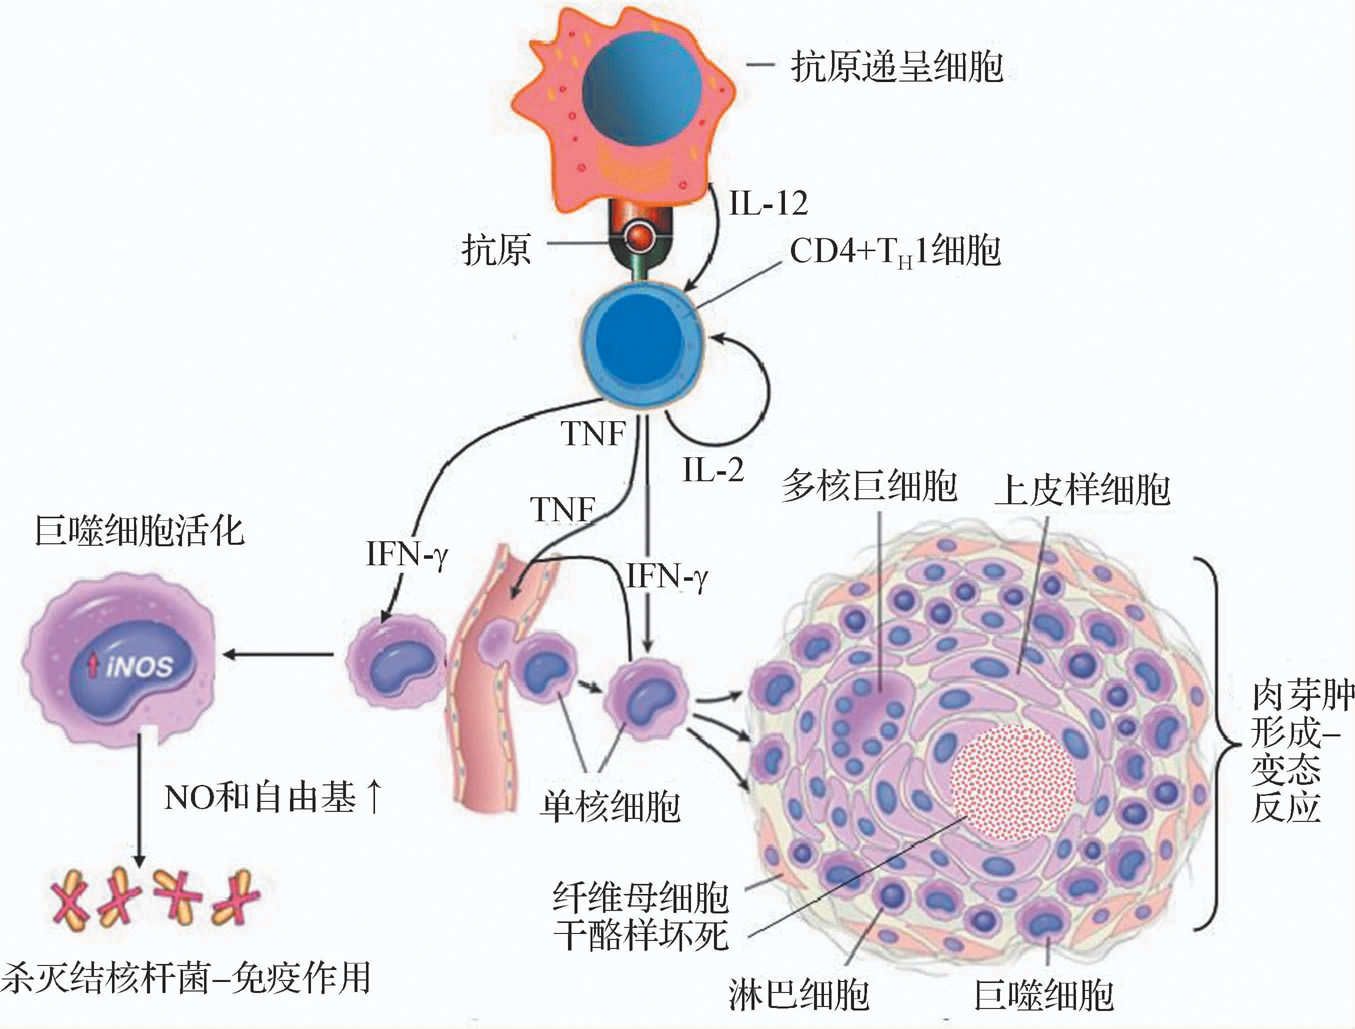
\includegraphics{./images/Image00224.jpg}
    \captionsetup{justification=centering}
    \caption{结核病发病机制模式图}
    \label{fig14-1}
\end{figure}
 
\begin{table}[ht]
	\caption{结核病基本病变与机体的免疫状态}
	\label{tab14-1}
	\centering
	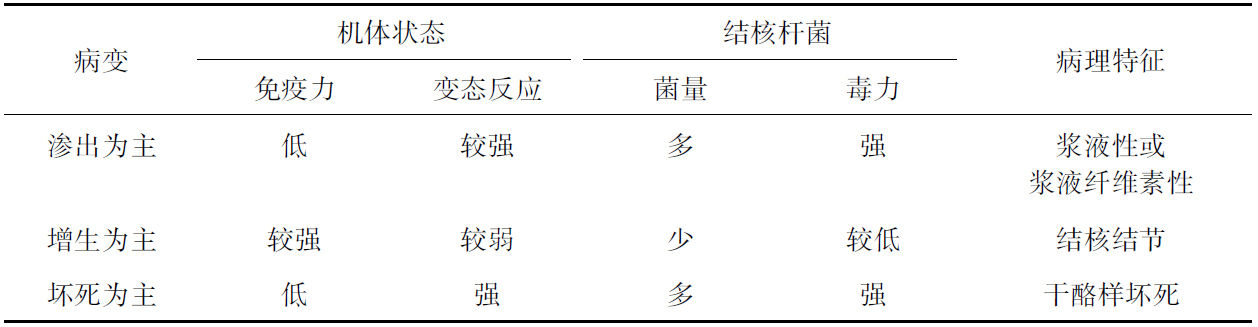
\includegraphics{./images/Image00225.jpg}
\end{table}


\subsubsection{结核病的基本病理变化}

结核杆菌在体内引起的病变具有一般炎症的变质、渗出和增生三种基本变化,但也有其特殊性。由于机体的免疫力和变态反应,细菌数量、毒力和组织特性的不同,结核病可有以下不同病变类型。

\paragraph{渗出为主的病变}
出现于结核性炎症早期或机体免疫力低下,细菌数量多、毒力强或变态反应较强时。好发于肺、浆膜、滑膜及脑膜等处。表现为浆液性或浆液纤维素性炎症。早期有中性白细胞浸润,继而由巨噬细胞取代。在渗出液和巨噬细胞内易查见结核杆菌。渗出性病变较不稳定,当机体抵抗力增强时,病变可完全吸收不留痕迹或转变为以增生为主的病变。恶化时较易转变为变质为主的病变。

\paragraph{增生为主的病变}
当细菌数量少,毒力较弱,或机体免疫反应较强时,则发生以增生为主的病变,形成特征性的结核结节(Tubercle,结核性肉芽肿)。结核结节是在细胞免疫的基础上形成的。当结核杆菌侵入人体后,最初出现的反应是中性白细胞浸润,它能活跃地吞噬但不能杀灭结核杆菌,24小时内即由巨噬细胞所取代。巨噬细胞主要来源于血液循环中的单核细胞,也可来源于结缔组织中的组织细胞,它能吞噬和杀灭结核杆菌。在结核杆菌菌体破坏后释放出的磷脂作用下,巨噬细胞体积增大,逐渐转变为类上皮细胞,其胞体呈梭形或多角形,胞浆丰富,淡伊红染,细胞境界不清,常以胞浆突起互相联络成片。多个类上皮细胞互相融合,或单个类上皮细胞经多次分裂形成多核巨细胞,称朗格汉斯巨细胞(Langhans'
giant
cell),细胞体积大,胞浆丰富,核数目多,排列在胞体的周边部呈花环状、马蹄形,或密集在胞体一端。典型的结核结节,由类上皮细胞、朗格汉斯巨细胞、外围淋巴细胞和少量反应性增生的成纤维细胞构成,中央有干酪样坏死(图\ref{fig14-2})。单个结核结节肉眼不易看见,当数个结节融合在一起,才形成肉眼可见的粟粒大小结节,其境界分明,灰白色,半透明,干酪样坏死多时呈现淡黄色,常隆起于脏器表面。

\begin{figure}[!htbp]
    \centering
    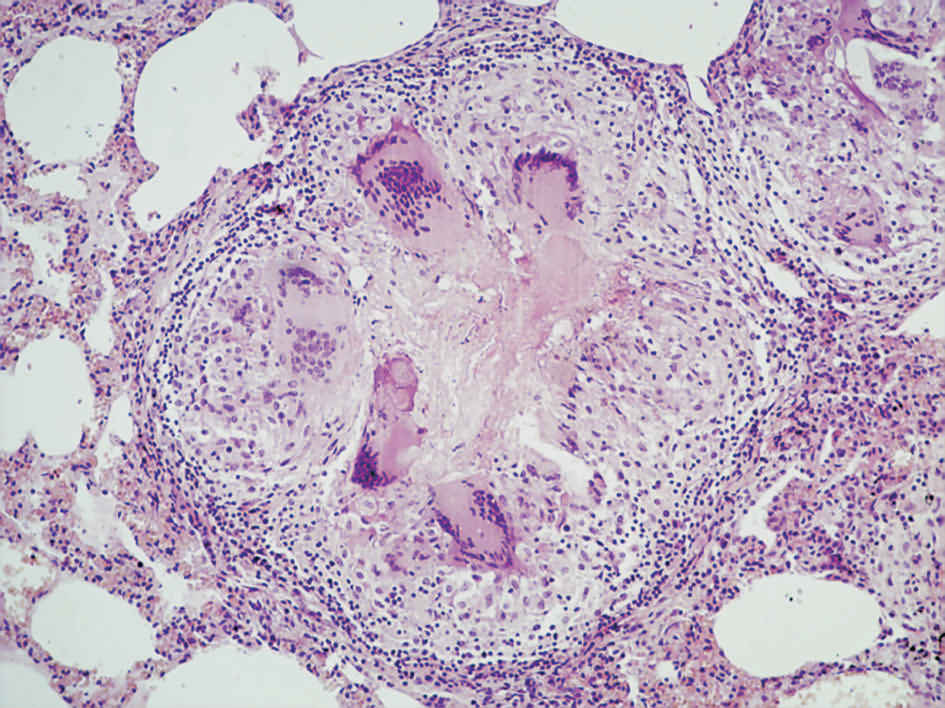
\includegraphics{./images/Image00226.jpg}
    \captionsetup{justification=centering}
    \caption{结核结节(HE染色,低倍)}
    \label{fig14-2}
\end{figure}

\paragraph{变质为主的病变}
在结核杆菌数量多,毒力强,机体抵抗力低下或变态反应较强烈等情况下,上述渗出性和增生性病变均可发生干酪样坏死,少数病变一开始就发生干酪样坏死。坏死组织因富含脂质而呈淡黄色、均匀细腻、质地松软、状似奶酪,故称干酪样坏死。镜下,坏死组织原组织结构轮廓消失,呈红染无结构的颗粒状物。新鲜干酪样坏死物中常会有数量不等的结核杆菌,而陈旧性病灶很难找到细菌。干酪样坏死的形态特征,特别是肉眼所见,对结核病的病理诊断具有一定的意义。

干酪样坏死灶内有多量抑制酶活性物质,因此可长期保持凝固性坏死状态。但有时在多种水解酶作用下,干酪样坏死灶也可发生软化和液化,形成半流体物质。液化有利于干酪样坏死排出,但更重要的是可成为结核杆菌在体内蔓延扩散来源,是结核病恶化进展的原因。

上述三种病变并不是孤立的,往往同时存在而以某一种病变为主,而且可互相转化。如以渗出为主的病变可因适当治疗和机体抵抗力增强而转化为增生为主的病变;反之,在机体抵抗力下降或变态反应增强时,原来增生为主病变可转化为渗出或变质为主病变,或原来渗出性病变转化为变质性病变。因此,结核病的受累器官或组织的病变常是复杂多样的。

\subsubsection{结核病基本病理变化的转化规律}

结核病的发展和结局取决于机体抵抗力和结核杆菌致病力之间的矛盾关系。在机体抵抗力增强时,结核杆菌被抑制、杀灭,病变转向愈合;反之,则转向恶化。

\paragraph{转向愈合}
(1)吸收消散:为渗出性病变的主要愈合方式,渗出物通过淋巴道和血道吸收,使病灶缩小或消散。较小范围干酪样坏死或增生性病变,经积极治疗,也可以吸收消散。X线检查时,可见边缘模糊、密度不匀、呈云絮状的渗出性病变的阴影,逐渐缩小或被分割成小片状,以至完全消失。临床称为吸收好转期。

(2)纤维化及钙化:增生性病变和小范围干酪样坏死灶可逐渐纤维化,最后形成瘢痕而愈合,较大的干酪样坏死则由其周边纤维组织增生形成纤维包裹,其中坏死物质逐渐干燥和钙化。但在被包裹、钙化的坏死灶中可有少量结核杆菌残留,当机体抵抗力下降时仍可复发进展。X线检查可见纤维化病灶呈边缘清楚、密度升高的条索状阴影,钙化为密度更高、边缘清晰的阴影。临床称为硬结钙化期。

\paragraph{转向恶化}
(1)浸润进展:结核病恶化时,病灶周围出现渗出性病变,病灶范围不断扩大,并继发干酪样坏死。X线检查,原病灶周围出现絮状阴影,边缘模糊。临床上称为浸润进展期。

(2)溶解播散:当病情继续恶化时,干酪样坏死物质可溶解液化,形成半流体物质,可经体内的自然管道排出,形成单个或多个、大小不一的空洞。坏死物中含有大量结核杆菌,既可通过自然管道播散到邻近部位而引起新的病灶,又可通过淋巴道和血道播散到全身,引起多个器官的结核病变。X线检查,可见病灶阴影密度深浅不一,出现透亮区(空洞)及大小不等的新的播散病灶阴影。临床称为溶解播散期。

\subsection{肺结核病}

结核病中最常见的是肺结核,主要是因结核分枝杆菌通过呼吸道感染。机体初次感染和再次感染结核菌的反应不同,肺部病变的发生和发展各有特点,所以肺结核病可分为原发性和继发性两大类。

\subsubsection{原发性肺结核病}

原发性肺结核病(primary pulmonary
tuberculosis)是指机体初次感染结核分枝杆菌后引起的肺部病变。儿童多见,故又称初染型肺结核病或儿童型肺结核病。偶见于未感染过结核杆菌的青少年或成人。

\paragraph{病理变化}
原发性肺结核病的病理形态特征是原发综合征形成。结核杆菌经呼吸道进入肺内,最先引起的肺部病变称为原发灶,原发灶多位于肺内通气较好肺上叶下部或下叶上部,靠近胸膜处,右侧肺更为多见。肉眼观:原发灶通常只有一个,呈圆形,直径多为1~1.5
cm,色灰黄。镜下观:初起为渗出性病变,继而发生干酪样坏死,周围形成结核性肉芽组织。由于是初次感染,机体缺乏对结核杆菌的免疫力,所以肺部结核病变不易局限,细菌可沿淋巴管播散到肺门淋巴结,引起结核性淋巴管炎和肺门淋巴结结核。后者表现为淋巴结肿大、干酪样坏死。

肺原发灶、结核性淋巴管炎和肺门淋巴结结核三者称为原发综合征(primary
complex)(图\ref{fig14-3})。X线检查呈哑铃状阴影。

\begin{figure}[!htbp]
    \centering
    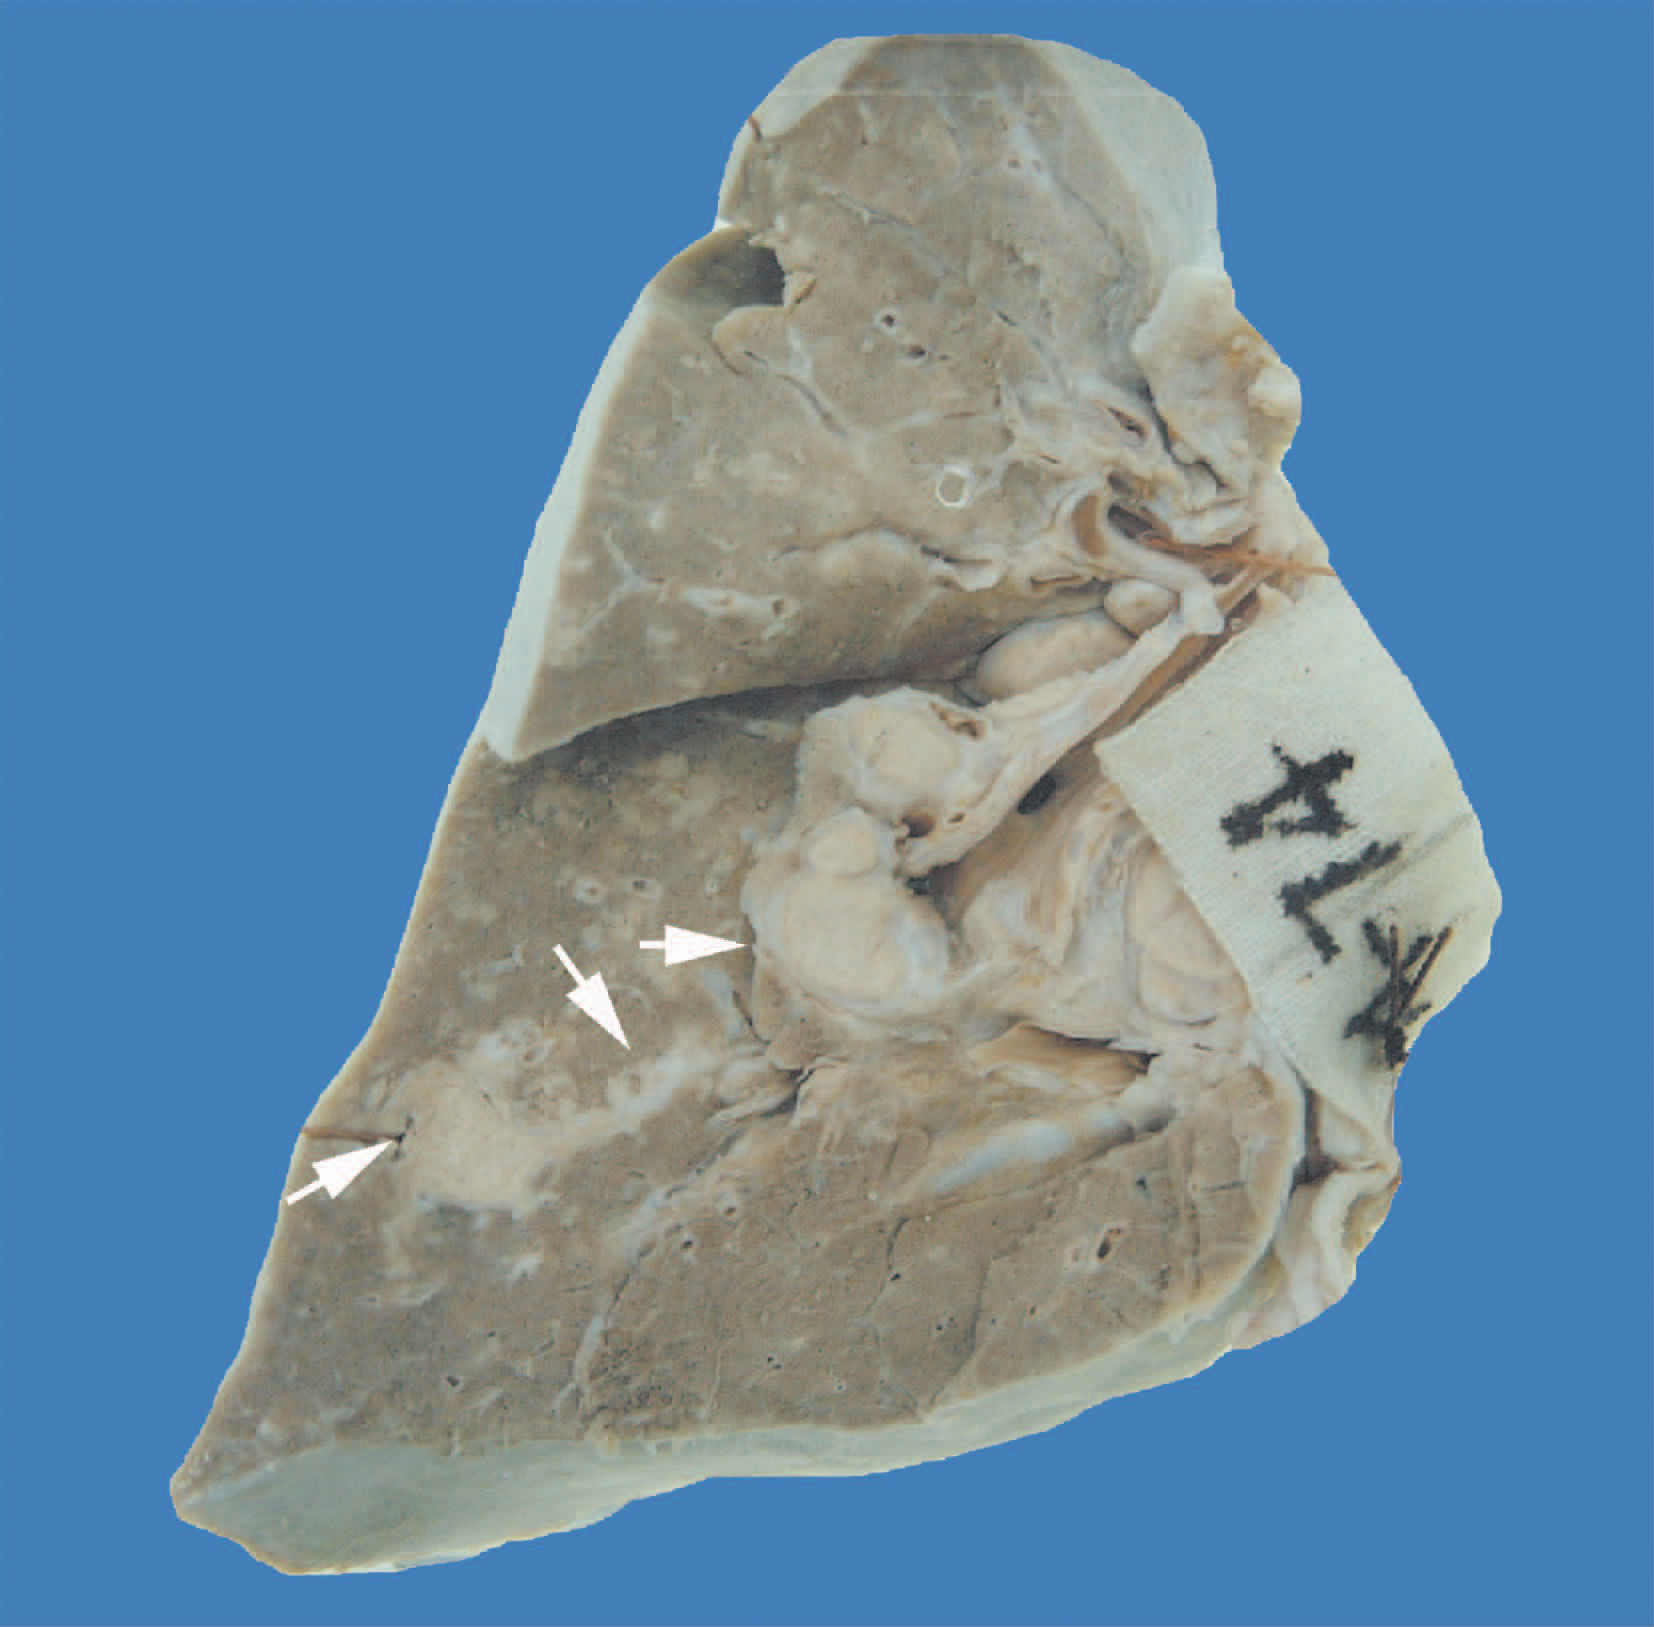
\includegraphics{./images/Image00227.jpg}
    \captionsetup{justification=centering}
    \caption{原发综合征\\ {\small 从左至右、白箭头分别指示原发灶、结核性淋巴管炎、肺门淋巴结结核}}
    \label{fig14-3}
\end{figure}

\paragraph{病变转归}
(1)痊愈:绝大多数(95%)原发性肺结核病,由于机体免疫力逐渐增强而自然痊愈,小的病灶可完全吸收或钙化,较大的病灶可发生纤维包裹或钙化。一般肺门淋巴结病变愈合较慢,有时肺内原发灶已愈合,而肺门淋巴结病变仍继续发展,蔓延到支气管淋巴结,形成支气管淋巴结结核,但经过适当治疗,这些病灶仍可被包裹、钙化或纤维化而痊愈。

(2)恶化:少数患者肺内和肺门的病灶恶化,通过支气管、淋巴道和血道而发生播散。病人常出现明显的低热、疲乏、盗汗、咳嗽等中毒症状。①支气管播散:肺原发病灶或肺门淋巴结的干酪样坏死范围不断扩大和液化后侵蚀了附近的支气管,通过支气管播散至同侧或对侧肺叶,形成干酪性肺炎(图\ref{fig14-4})。②淋巴道播散:肺门淋巴结结核,可沿淋巴管播散到支气管、气管分叉处、气管旁、纵隔、锁骨上下的淋巴结和颈部的淋巴结等。③血道播散:当机体免疫力较差,结核杆菌可直接侵入肺静脉及其分支,引起血行播散性结核病。大量结核杆菌在短时间内侵入肺静脉,经左心至大循环,播散到全身各器官,如肺、肝、脑、脾、肾和骨髓等处,全身各器官均匀密布粟粒大小、灰白色、境界清楚的圆形小结节(直径为1~2
mm),称急性全身性粟粒性结核病。临床上病情危重,有高热、寒战等中毒症状。如结核杆菌少量多次进入血流,先后在全身不同组织、器官发生大小不等、新旧不一的病变,称慢性全身性粟粒性结核病。偶尔病变也可仅局限于肺内。当干酪样坏死液化后破入附近体静脉系统,或因含有大量结核杆菌的淋巴液由胸导管回流,经静脉入右心,沿肺动脉播散于两肺。如大量结核杆菌在短时间内侵入肺内,则为急性粟粒性肺结核,它常是急性全身性粟粒性结核病的一部分。如结核杆菌小量多次进入肺内,则为慢性粟粒性肺结核。后者多发生于有一定免疫力的成人,原发灶已痊愈,结核杆菌由肺外器官的结核病灶间歇入血,播散于肺内,形成新旧不一、大小不等的病灶,以增生性病变为主。临床病程较长。

\begin{figure}[!htbp]
    \centering
    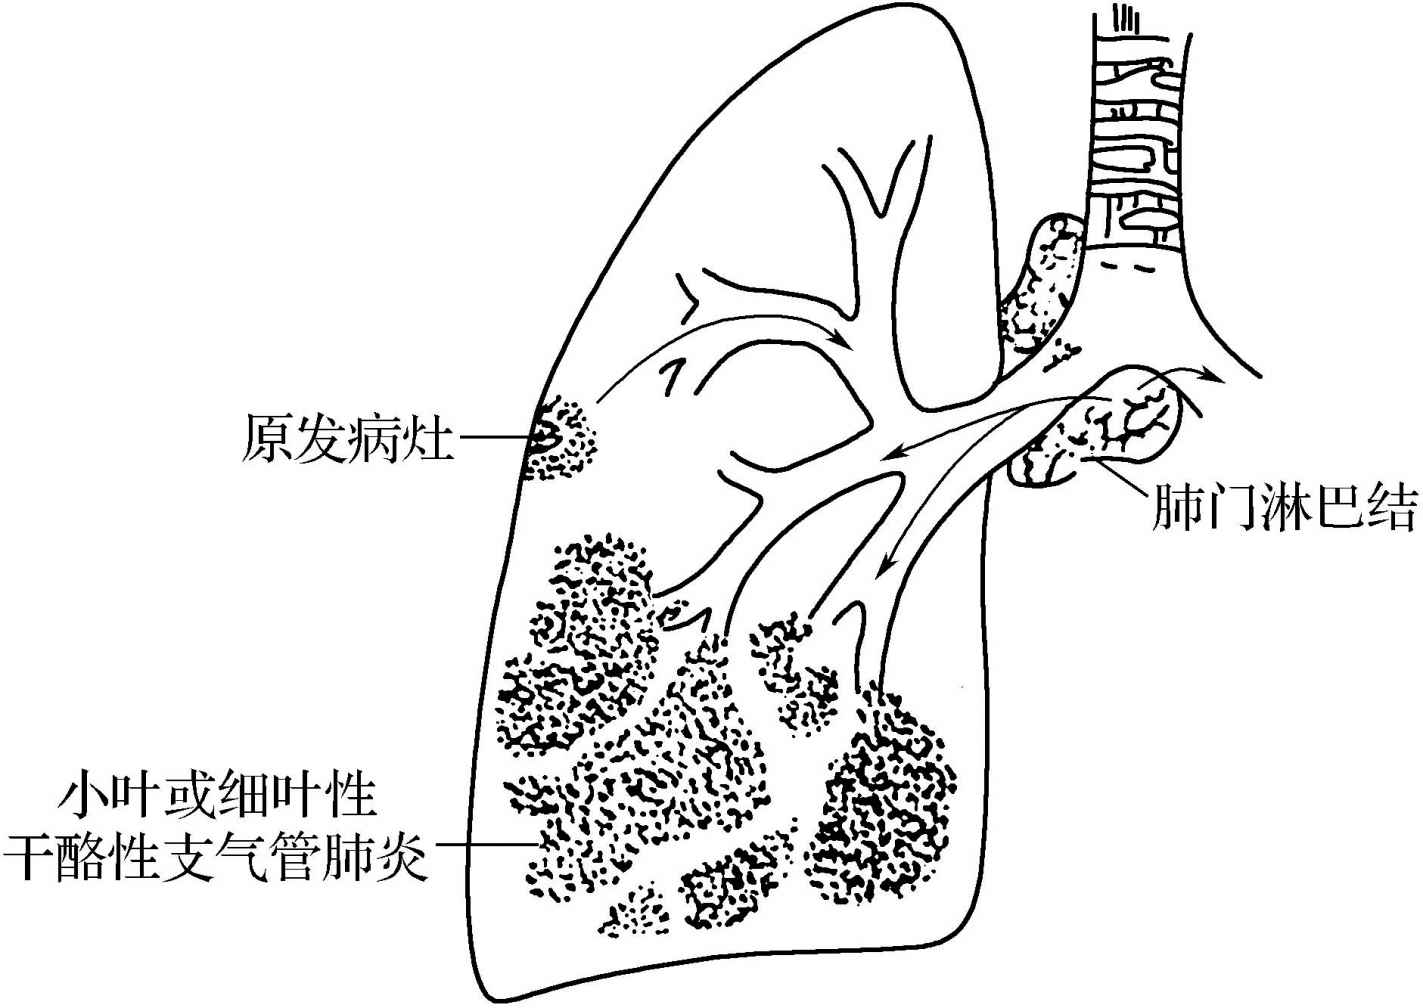
\includegraphics{./images/Image00228.jpg}
    \captionsetup{justification=centering}
    \caption{原发性肺结核沿支气管播散}
    \label{fig14-4}
\end{figure}

\subsubsection{继发性肺结核病}

继发性肺结核病(secondary pulmonary
tuberculosis)是指机体再次感染结核杆菌所致的肺结核病。多见于成人,故又称为成人型肺结核病。再次感染的细菌可能有两种来源:一是外源性感染,由体外分枝结核杆菌再次感染所致,与原发性肺结核无关;二是内源性感染,即分枝结核杆菌潜伏在体内的原有病灶中,当机体抵抗力下降时,病灶发展为继发性肺结核病。

继发性肺结核病患者对结核分枝杆菌已有一定的免疫力,故病变一般局限,因而其病变与原发性肺结核病有以下不同特点:①病变多从肺尖开始,尤以右肺尖多见。这可能与人体直立时肺尖的动脉压较低,血循环较差,通气不畅,而使局部组织抵抗力减弱,细菌易在该处繁殖有关;②病变以干酪样坏死及增生为主。由于变态反应,病变发展迅速而且剧烈,易发生干酪样坏死,同时机体已产生较强免疫力,坏死周围病变多以增生为主,形成结核结节;③播散方式主要通过支气管播散。结核杆菌不易侵入血道或淋巴道,因此,肺门淋巴结一般无明显病变,经血道播散引起全身性粟粒性结核病也较少见;④病程长病变复杂。病变常随机体抵抗力的消长而变化,时好时坏,有时以增生为主,有时以渗出、变质为主。因此,肺内病变轻重不一,新旧病变交错存在。

继发性肺结核病根据其病变特点和临床经过,可分为以下几种主要类型。

\paragraph{局灶型肺结核}
是继发性肺结核的早期病变,病变多位于肺尖下2~4
cm处,直径一般为0.5~1
cm。病灶可为一个或数个,多以增生性病变为主,中央可发生干酪样坏死。多数情况下,病灶易局限,发生纤维化、钙化而愈合。X线检查显示肺尖部有单个或多个境界清楚的结节状阴影。临床上患者常无明显自觉症状,多在体检时发现,属非活动性肺结核病。当患者抵抗力下降时,可发展为浸润型。

\paragraph{浸润型肺结核}
此型是成人结核病中最常见的类型,也是临床上最常见的活动性肺结核病。大多数是由局灶型肺结核发展而来,少数一开始即为浸润型。病灶常位于肺尖部或肺尖下部,右肺多见。病变多以渗出性改变为主。镜下观:肺泡腔内有大量浆液、纤维素、淋巴细胞、单核细胞和少量中性白细胞,病灶中央可有不同程度的干酪样坏死。X线检查,可见肺上部锁骨下区出现边缘模糊的片状云絮状阴影,亦称锁骨下浸润。临床上本病多见于青年人,常有午后低热、盗汗、乏力、咳嗽、咯血等症状,痰中可查见结核分枝杆菌。如及时适当治疗,渗出性病变可完全或部分吸收,病灶缩小,或转变为增生性病变,通过纤维化,包裹和钙化而愈合。如病人抵抗力差或未能及时治疗,病情继续发展,渗出性病灶和干酪样坏死灶不断扩大,液化的干酪样坏死经支气管排出后可形成急性空洞。如空洞壁不规则,内表面及洞壁均为干酪样坏死物质者称为无壁空洞,如果外有薄层结核性肉芽组织形成者称为薄壁空洞。空洞一般较小,内壁坏死层中有大量结核杆菌,经支气管播散可引起干酪性肺炎;如经及时有效的抗结核治疗,洞壁内肉芽组织增生,可使洞腔逐渐缩小,最终形成瘢痕组织而愈合;空洞也可塌陷,形成索状瘢痕组织而愈合;急性空洞经久不愈,则可发展为慢性纤维空洞型肺结核。

\paragraph{慢性纤维空洞型肺结核}
多由浸润型肺结核经久不愈发展而来,是成人慢性肺结核病的常见类型。病变有以下特点:①肺内有一个或多个厚壁空洞形成,多位于肺上叶,大小不等,形状不规则。壁厚可达1
cm以上。镜下空洞壁分三层:内层为干酪样坏死物,其中有大量结核菌;中层为结核性肉芽组织;外层为纤维结缔组织。②单侧或双侧肺组织内,由于空洞内的干酪样坏死液化物不断地通过支气管在肺内播散,形成新旧不一、大小不等、病变类型不同的病灶,病变呈复杂多样化(图\ref{fig14-5})。因空洞壁厚而且长期存在,空洞与支气管相通,咳出含菌的痰经过呼吸道时可引起气管或喉结核,被咽下可引起肠结核,排出体外又成为结核病传染源,故此型又称开放性结核。如肺内血管被侵蚀,可咯血。③严重的慢性纤维空洞型肺结核,由于病变长期迁延反复,肺组织遭受严重破坏,引起广泛纤维化,使肺体积缩小、变形、变硬,胸膜广泛增厚并与胸壁粘连,成为硬化型肺结核,严重影响肺功能。肺广泛纤维化还可导致肺循环阻力增高,肺动脉高压,进而引起肺源性心脏病。

近年来,广泛采用多药联合抗结核治疗及增加机体抵抗力的措施,较小的空洞可被纤维组织充填,最后瘢痕愈合。较大的空洞内壁坏死组织脱落净化、洞壁的结核性肉芽组织逐渐转变为纤维瘢痕组织,并通过邻近支气管上皮增生或化生为鳞状上皮,覆盖空洞内壁,形成空洞仍存在的所谓“开放性愈合”。

\begin{figure}[!htbp]
    \centering
    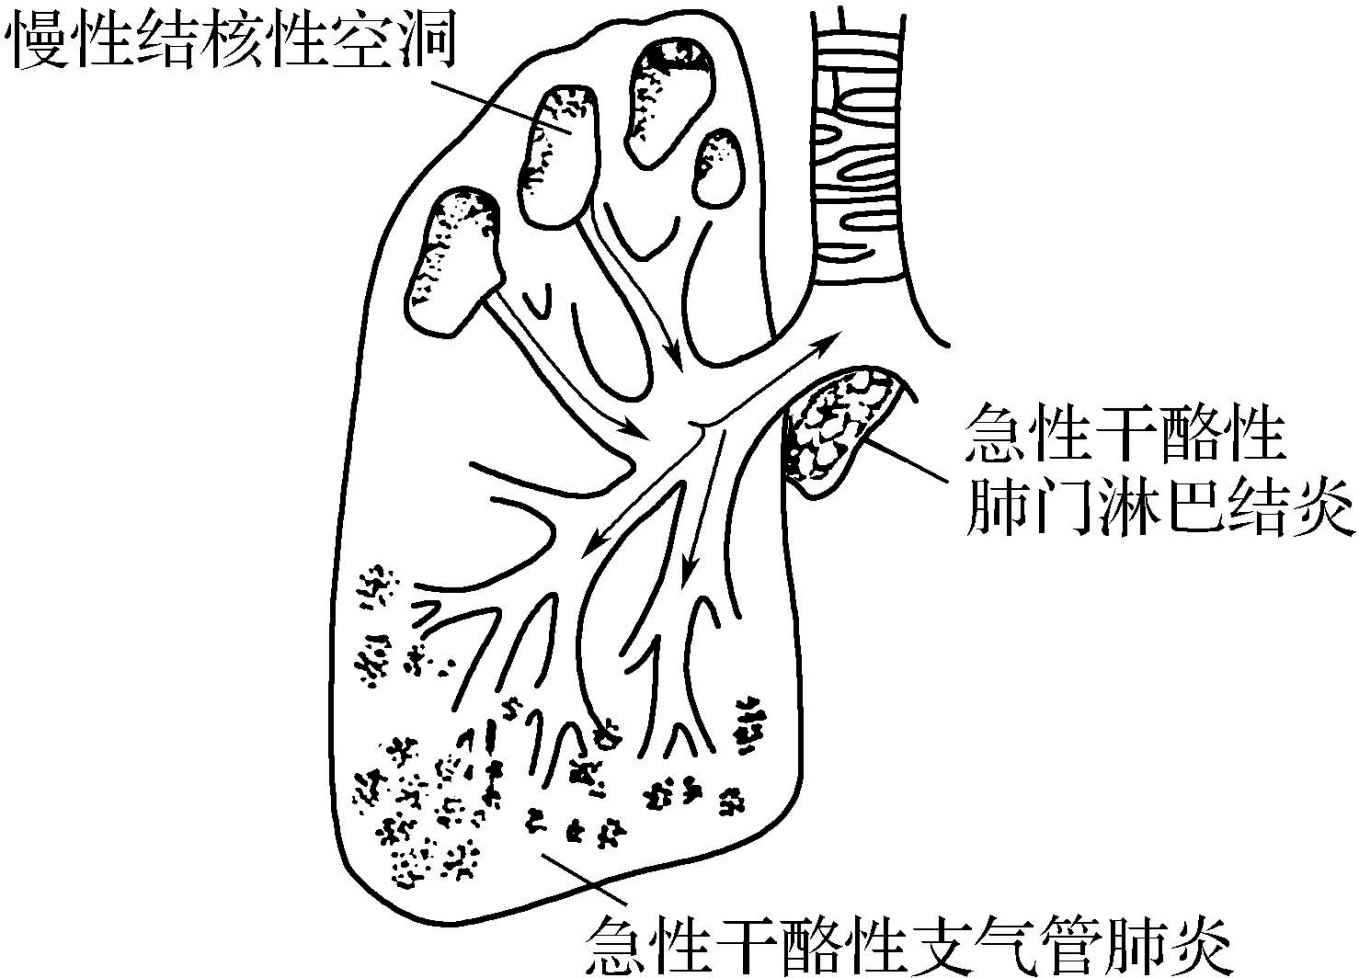
\includegraphics{./images/Image00229.jpg}
    \captionsetup{justification=centering}
    \caption{慢性纤维空洞型肺结核}
    \label{fig14-5}
\end{figure}

\paragraph{干酪性肺炎}
是浸润型肺结核最严重的一类,常发生在机体抵抗力差,对结核杆菌敏感性过高的病人。多由浸润型肺结核恶化进展而来,或由空洞内液化的干酪样坏死物经支气管播散所致。病变处为广泛性渗出性改变,并很快发生干酪样坏死。按病变范围可分为大叶性或小叶性干酪性肺炎。肉眼观:病变肺叶肿大实变,切面呈黄色干酪样,常见多个薄壁空洞,并可互相融合。镜下观:肺泡腔内有显著的浆液、纤维素性渗出物,内含大量巨噬细胞、淋巴细胞,并见广泛的干酪样坏死物,其中可查见大量抗酸染色阳性的结核杆菌。患者常有严重的中毒症状,表现为长期高热、寒战、咯血等。病情发展迅猛,病死率高,故有“百日痨”或“奔马痨”之称。本型目前已经罕见。

{5.结核球(tuberculoma)}
又称结核瘤,是孤立的、有纤维组织包裹的、境界分明的球形干酪样坏死灶,直径为2~5
cm。常位于肺上叶,多为单个。切面灰白色、质松软,常呈同心圆状结构,并可见点状钙化灶(图\ref{fig14-6})。结核球可来自:①浸润型肺结核的干酪样坏死灶纤维包裹发展而成;②空洞引流的支气管阻塞后,干酪样坏死物充填空洞形成;③或是多个干酪样坏死病灶融合而成。结核球是相对静止的病变,可保持多年无进展;或发生机化或钙化而愈合;亦可恶化进展,如干酪样坏死灶扩大、液化,包膜溃破,甚至形成空洞。因结核球有纤维组织包裹,药物不易发挥作用,故临床上多采取手术切除治疗。

\begin{figure}[!htbp]
    \centering
    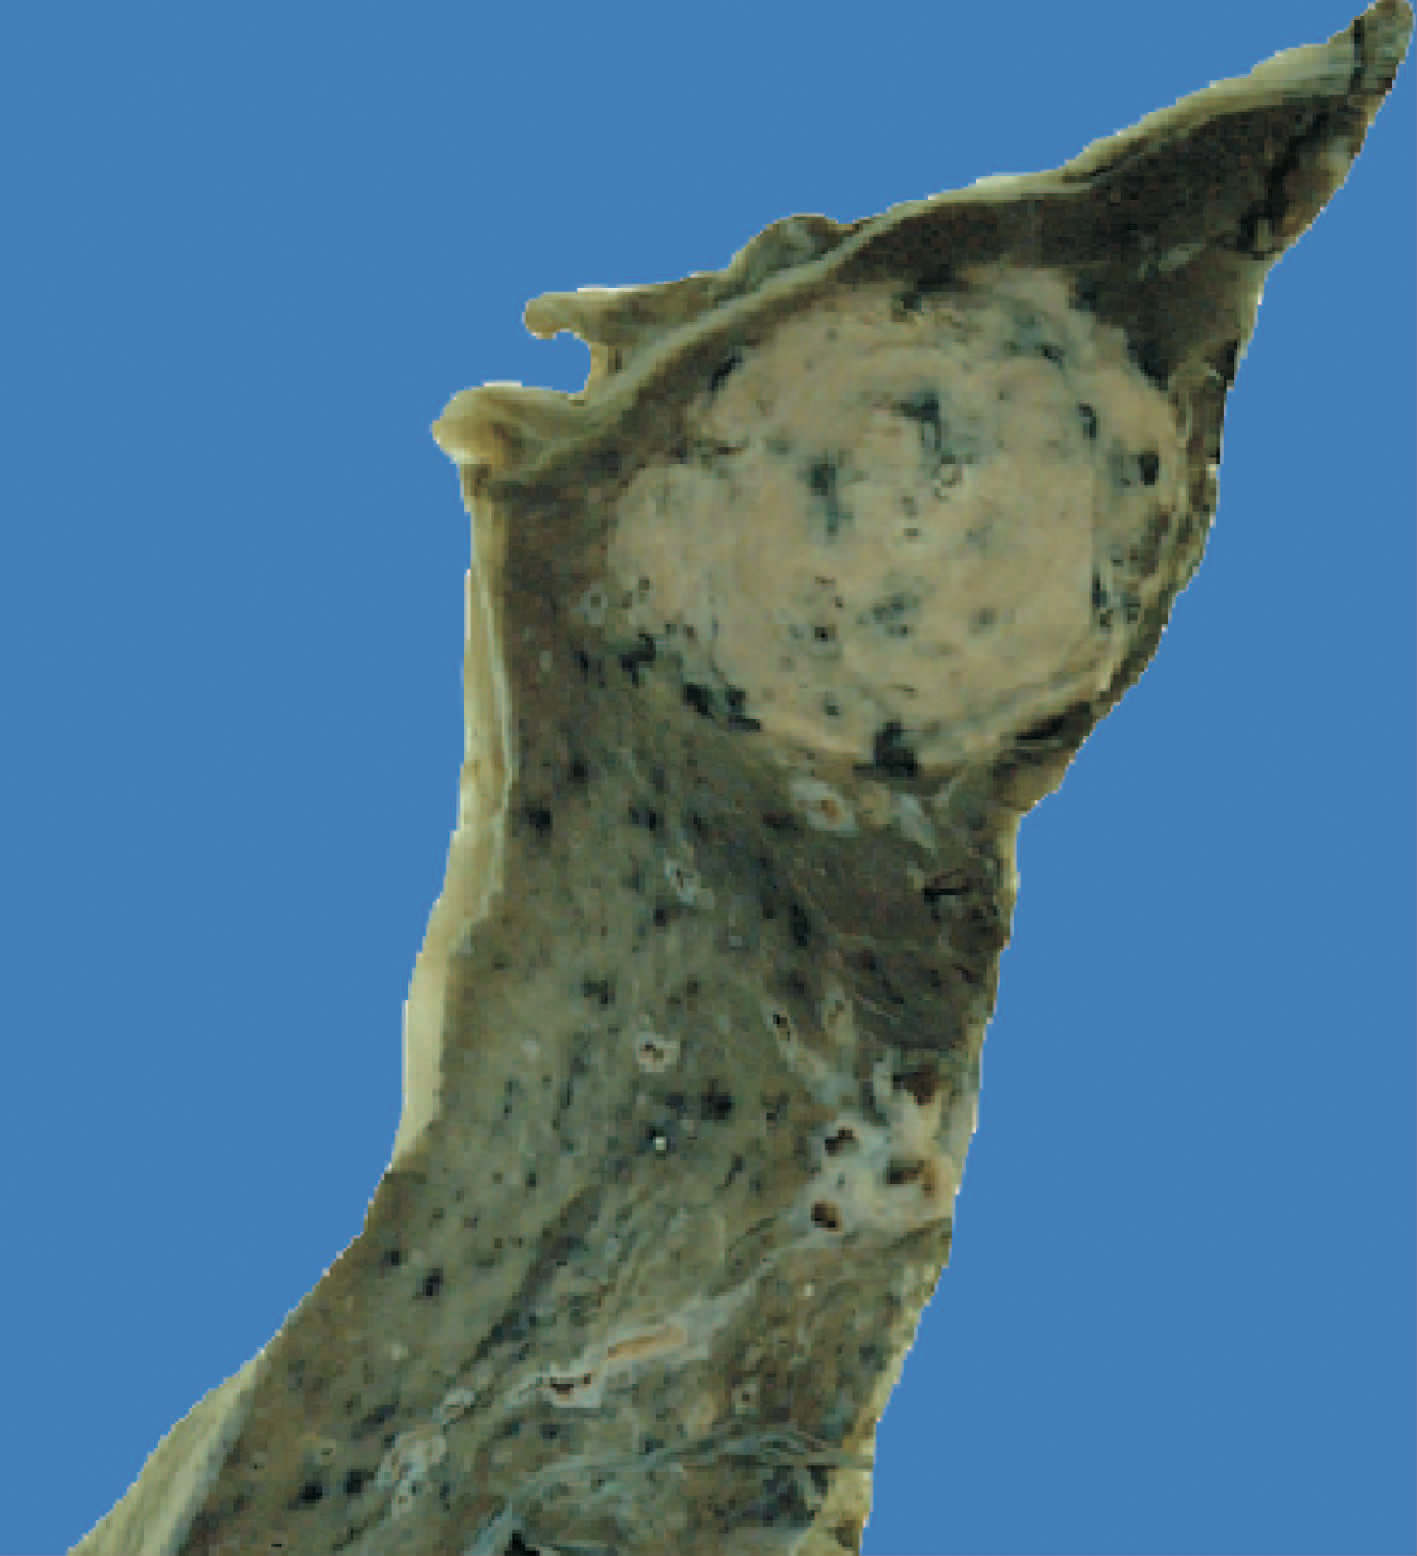
\includegraphics{./images/Image00230.jpg}
    \captionsetup{justification=centering}
    \caption{结核球}
    \label{fig14-6}
\end{figure}

\paragraph{结核性胸膜炎}
在原发性或继发性肺结核病的不同时期均可发生,多见于青年人,结核性胸膜炎按病变性质常分为湿性和干性两种。

(1)湿性结核性胸膜炎(又称渗出性结核性胸膜炎):较为多见,大多发生于原发性肺结核病的过程中,为肺内原发病灶或肺门淋巴结病灶的结核菌播散至胸膜引起,或是对弥散至胸膜的菌体蛋白发生的变态反应。病变主要为浆液、纤维素性炎。胸膜充血,胸膜腔内有浆液、淋巴细胞和纤维素渗出,有时有较多的红细胞及脱落的间皮细胞,但结核杆菌难以查见。临床上常表现为胸痛,出现胸膜摩擦音及胸腔积液的体征。经适当治疗,一般渗出性胸膜炎可完全吸收而痊愈。如渗出物中纤维素过多不易吸收,则可发生机化,使胸膜增厚并发生粘连。

(2)干性结核性胸膜炎(又称增生性结核性胸膜炎):较为少见,多由靠近胸膜的肺结核病灶直接蔓延所致。常发生于肺尖,病变比较局限,以增生改变为主,浆液渗出较少,一般通过纤维化而痊愈,并常使局部胸膜增厚和粘连。

原发性肺结核与继发性肺结核既有联系又有区别,在许多方面有不同的特征(表\ref{tab14-2},图\ref{fig14-7})。

\begin{table}[ht]
	\caption{原发性和继发性肺结核病比较表}
	\label{tab14-2}
	\centering
	\begin{tabular}{lll}
	\toprule
	&原发性肺结核病&继发性肺结核病\\
	\midrule
	结核杆菌感染&初次&再次\\
发病人群&儿童&成人\\
对结核杆菌的免疫力或过敏性&无&有\\
病理特征&原发综合征&病变多样化,新旧病灶复杂,较局限\\
起始病灶&上叶下部、下叶上部近胸膜处&肺尖部\\
主要播散途径&淋巴道或血道&支气管\\
病程&短,大多自愈&长,需治疗\\
	\bottomrule
	\end{tabular}
\end{table}




\begin{figure}[!htbp]
    \centering
    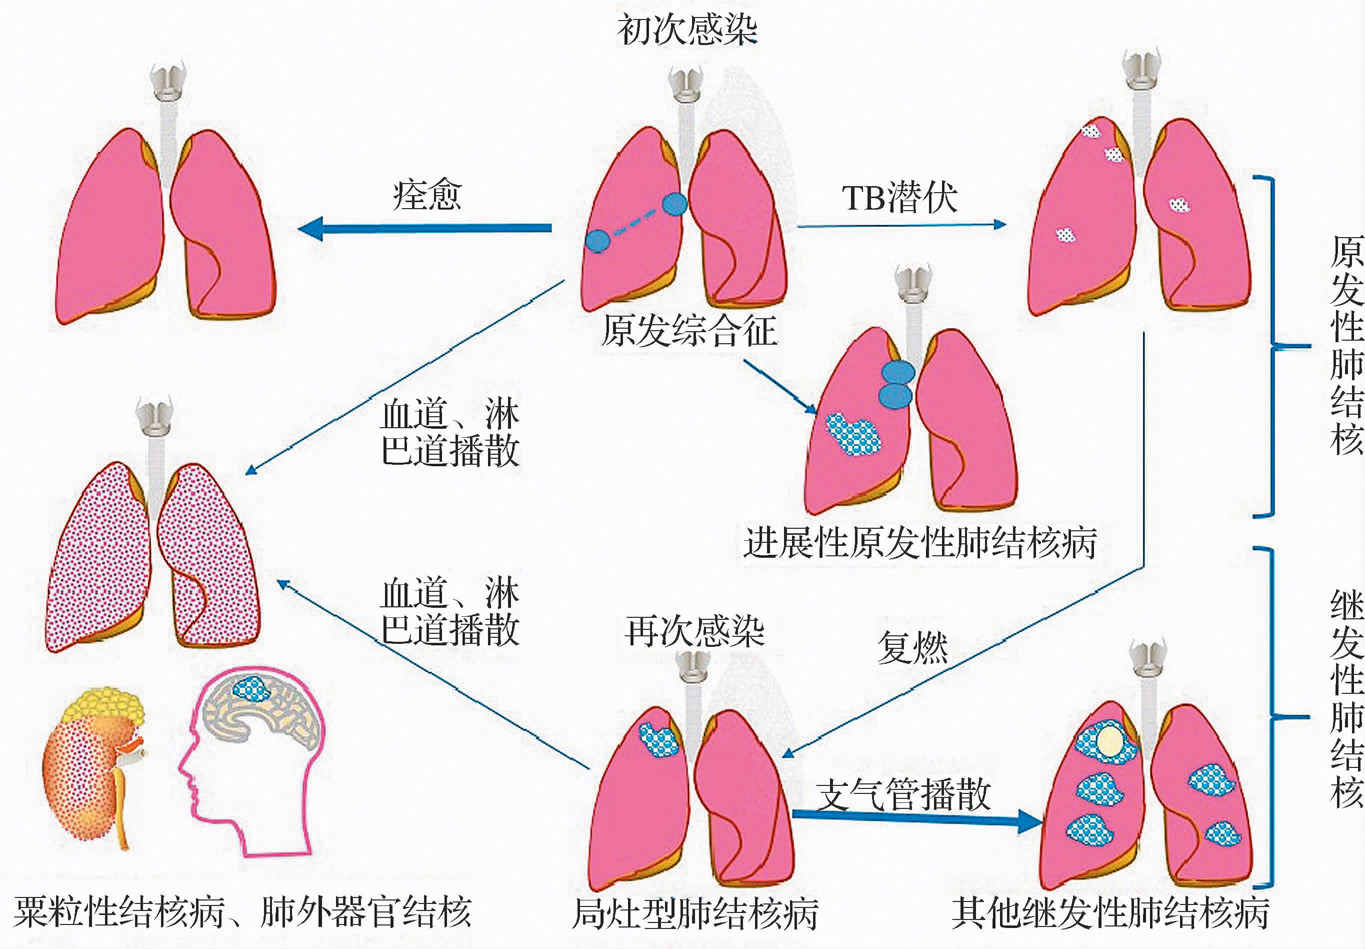
\includegraphics{./images/Image00232.jpg}
    \captionsetup{justification=centering}
    \caption{原发性肺结核与继发性肺结核主要发展变化过程示意图}
    \label{fig14-7}
\end{figure}

\subsection{肺外器官结核病}

肺外器官结核病(extrapulmonary
tuberculosis)是指肺以外各器官所发生的结核病。大多为原发性肺结核病的结核分枝杆菌经血行播散和淋巴道播散到肺外器官引起。常见有肠、腹膜、肾、生殖腺、脑膜、骨和关节等脏器。

\subsubsection{肠结核病}

肠结核病(intestinal
tuberculosis)可分为原发性和继发性两种类型。原发性肠结核较少见,多见于儿童,一般因食入含结核杆菌牛奶或乳制品而感染。细菌进入肠壁,在肠黏膜形成原发性结核病灶,继而细菌侵入淋巴管循淋巴流到达肠系膜淋巴结,形成与原发性肺结核病相似的肠原发综合病灶。绝大多数肠结核继发于活动性空洞型肺结核,由于反复咽下含菌痰液而引起。好发于回盲部,这可能是因为结核杆菌易侵犯淋巴组织,而回盲部肠壁淋巴组织较丰富;加之食物在回盲部滞留时间较长,此处肠管蠕动与逆蠕动较强,易引起肠组织机械性损伤,从而使结核杆菌有更多机会进入肠壁,引发肠结核病。继发性肠结核根据病变特点可分为溃疡型和增生型两种。

\paragraph{溃疡型}
此型较多见。早期结核杆菌由胸壁黏膜上皮进入肠壁淋巴组织,引起结核结节形成并互相融合,以后发生干酪样坏死,溃破脱落而形成溃疡。由于细菌沿肠壁环形淋巴管蔓延,病变不断扩大,因此溃疡常呈环形腰带状,与肠管长轴垂直。溃疡一般较浅,边缘参差不齐如鼠咬状(图\ref{fig14-8})。底部附着有干酪样坏死物,其下为结核性肉芽组织。浆膜面充血,常有纤维素渗出,并可见有灰白色的结核结节沿肠壁淋巴管呈线形排列,受累的浆膜层常与邻近组织粘连。临床上表现为慢性腹痛、腹泻、营养障碍等。溃疡愈合后,由于瘢痕组织收缩可引起肠腔狭窄。

\paragraph{增生型}
较为少见。以增生性病变为主,病变特征是肠壁内有大量结核性肉芽组织形成和纤维组织显著增生,使肠壁增厚、变硬、肠腔狭窄。黏膜表面可有浅溃疡及息肉形成。临床上表现为慢性不完全性低位肠梗阻症状,右下腹常可触及肿块,应与肿瘤鉴别。

\begin{figure}[!htbp]
    \centering
    
\includegraphics{./images/Image00233.jpg}
    \captionsetup{justification=centering}
    \caption{肠结核\\ {\small 可见与肠管长轴垂直之溃疡,边缘不整齐}}
    \label{fig14-8}
\end{figure}

\subsubsection{结核性腹膜炎}

结核性腹膜炎(tuberculous
peritonitis)多见于青少年。感染途径以腹腔内结核病灶直接蔓延为主。通常继发于肠结核、肠系膜淋巴结结核或输卵管结核。由腹膜外结核灶经血行播散至腹膜者少见。根据病变特点可分为干性和湿性两型,但大多为混合型。典型的湿性型常有大量的腹腔积液,积液为浆液纤维素,有时亦可是血性。干性结核性腹膜炎因有大量纤维素渗出机化而引起腹腔脏器粘连。

\subsubsection{结核性脑膜炎}

结核性脑膜炎(tuberculous
meningitis)多见于儿童,成人少见。主要是原发性肺结核病血道播散所致,常为全身粟粒性结核病的一部分。成人的肺及肺外结核病的晚期亦可经血行播散引起。部分病例也可由脑实质内的结核病灶液化、破溃,大量结核杆菌直接进入蛛网膜下腔所致。

病变以脑底部最明显,在桥脑、脚间池、视神经交叉及大脑外侧裂等处之蛛网膜下腔内,可见有大量灰黄色混浊的胶冻样渗出物积聚。脑室脉络丛及室管膜有时也有灰白色结核结节形成。病变严重者可累及脑皮质而引起脑膜脑炎。病程长者则可发生闭塞性血管内膜炎,从而可引起多发性脑软化。未经适当治疗致病程迁延的病例,由于蛛网膜下腔渗出物的机化而发生粘连,可使第四脑室中孔和外侧孔堵塞,引起脑积水并发症。

\subsubsection{泌尿生殖系统结核病}

\paragraph{肾结核病}
患者常为男性青壮年(20~40岁)。肾结核发病多为单侧,病原菌来自于肺结核病灶的血道播散所致。病变大多起始于肾皮质、髓质交界或肾锥体乳头处。最初为局灶性结核病变,继而发生干酪样坏死,然后破坏肾乳头,崩溃入肾盂,形成结核性空洞。随着病变的不断扩展蔓延,肾内形成多个结核空洞,最终使肾脏全部被毁仅剩一空壳,肾功能丧失。同时,干酪样坏死物随尿液下行,使输尿管和膀胱相继感染受累。输尿管黏膜可发生溃疡,结核性肉芽组织形成并纤维化,使输尿管管壁增厚变硬、管腔狭窄,甚至阻塞而引起肾积水或积脓。病变进一步累及膀胱三角区,黏膜发生结核性溃疡,最后累及整个膀胱,膀胱因纤维化而容积缩小,并引起对侧肾盂积水。在男性尚可累及前列腺、精索等。临床上可出现尿频、尿急、血尿、脓尿等症状。如两侧肾脏严重受损,可引起肾功能不全。

\paragraph{生殖系统结核病}
男性生殖系统结核病与泌尿系统结核病有密切关系,结核杆菌可使前列腺、精囊感染,并可蔓延波及输精管、附睾等处,血道感染少见。病变部位有结核结节形成和干酪样坏死,最常见于附睾,表现为附睾肿大变硬、疼痛,并可与阴囊粘连,溃破后引起长期不愈的窦道。

女性生殖系统结核病,主要由血道或淋巴道播散而来,亦可由邻近器官结核病直接蔓延而来,多见于输卵管,其次为子宫内膜、卵巢,是导致女性不孕的重要原因。

\subsubsection{骨与关节结核}

骨及关节结核病多由原发综合征病灶的血道播散而来,多见于儿童和青少年,因此时正处骨发育的旺盛时期,骨内血管丰富,感染机会较多。骨结核多侵犯脊椎骨、指骨及长骨骨骺(如股骨下端和胫骨上端)。关节结核以髋、膝、踝、肘等处关节多见。

\paragraph{骨结核}
病变常起始于骨骺松质骨内,以后病变继续发展成为干酪样坏死型和增生型。以干酪样坏死型多见,其特点是病变部位干酪样坏死明显,骨质被破坏形成死骨,周围软组织亦常受累,形成结核性肉芽组织及干酪样坏死。坏死物液化可在骨旁形成“结核性脓肿”,由于此脓肿局部无红、热、痛表现,故名“冷脓肿”(cold
abscess)。脓肿穿破皮肤,可形成经久不愈的窦道。增生型较少见,主要形成结核性肉芽组织,病灶内骨小梁被侵蚀、吸收和消失,无明显干酪样坏死及死骨形成。

脊椎结核病是骨结核病中最常见一种,多发生于第10胸椎至第2腰椎,椎体常发生干酪样坏死,并累及椎间盘和邻近椎体。由于病变椎体不能负重,从而引起椎体塌陷造成脊椎后凸畸形(图\ref{fig14-9})。如病灶穿破骨皮质,侵犯周围软组织,干酪样坏死物液化后可在局部形成结核性脓肿,其液化的干酪样坏死物亦可沿筋膜间隙向下流注,在远隔部位形成“冷脓肿”。如腰椎结核可在腰大肌鞘膜下、腹股沟韧带下及大腿部形成“冷脓肿”。由于脊椎后凸和椎旁结核性肉芽组织或“冷脓肿”压迫脊髓,可致截瘫。

\begin{figure}[!htbp]
    \centering
    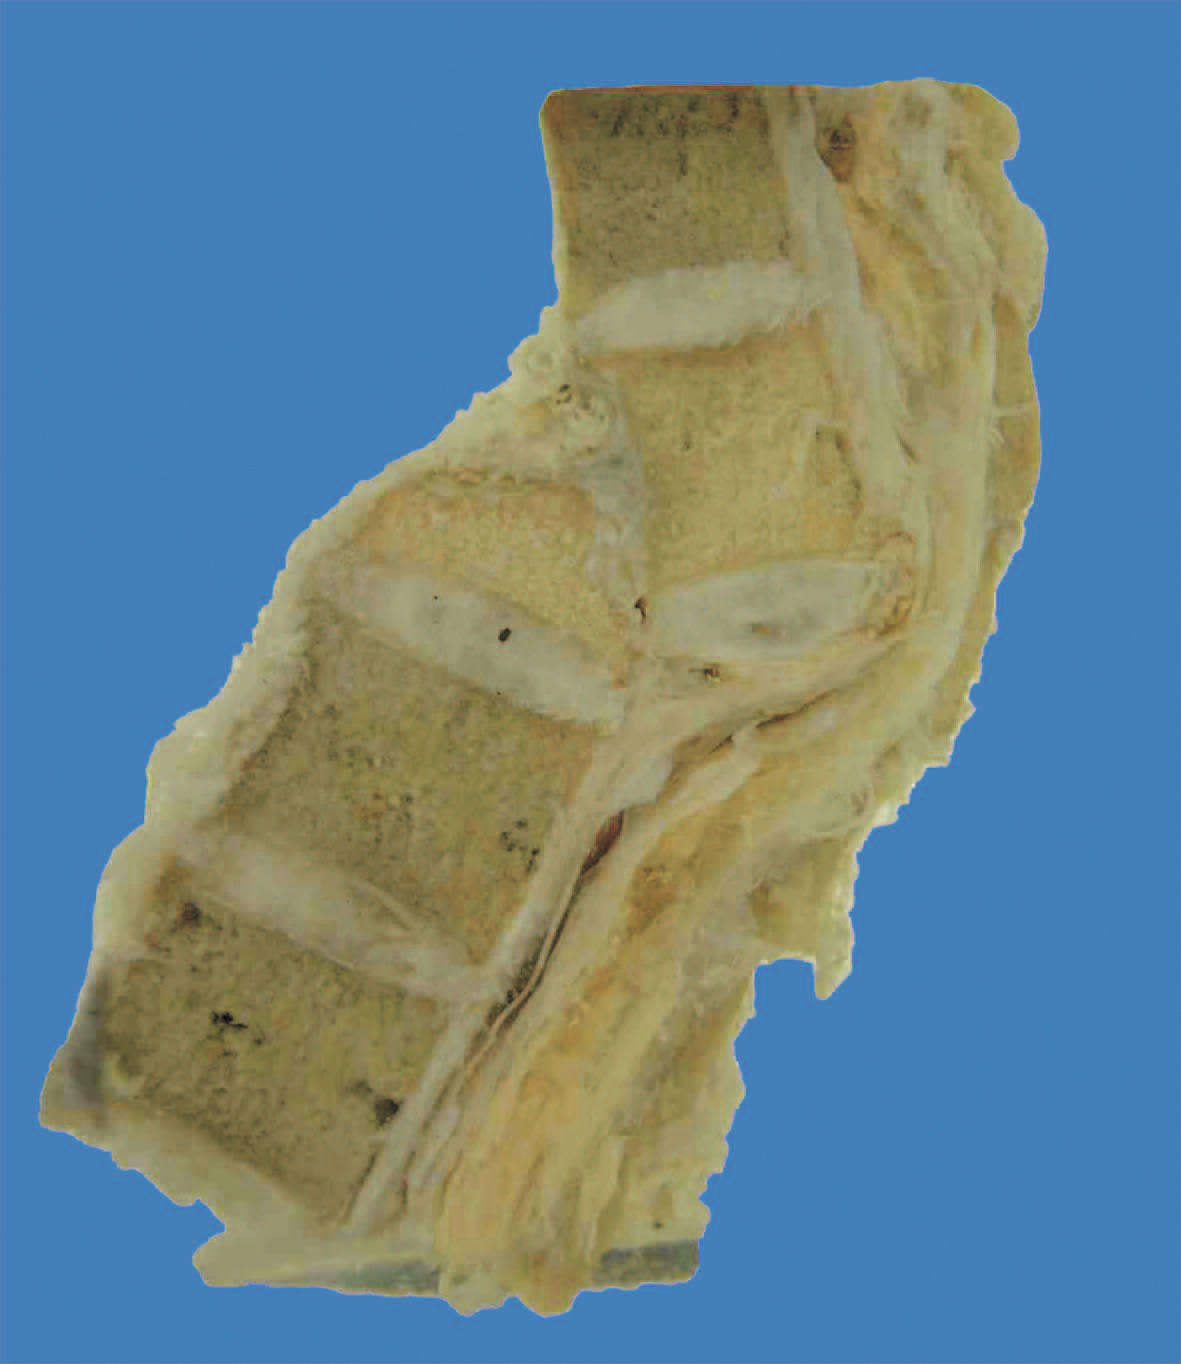
\includegraphics{./images/Image00234.jpg}
    \captionsetup{justification=centering}
    \caption{脊椎结核}
    \label{fig14-9}
\end{figure}

\paragraph{关节结核}
常继发于骨结核,病变通常开始于骨骺或干骺端,发生干酪样坏死。累及关节软骨及滑膜时即成为关节结核。病变形成结核性肉芽组织,关节软骨破坏,滑膜增厚,关节腔内有浆液、纤维素性渗出物。关节周围软组织炎性水肿和慢性炎症,致关节肿胀。如病变累及软组织和皮肤,穿破皮肤形成窦道。病变愈合时,关节因纤维化而粘连,从而使关节僵直、畸形、失去正常的运动功能。

\subsubsection{淋巴结结核病}

淋巴结结核病常见于儿童和青年。病变常累及颈部、肺门、支气管和肠系膜淋巴结,尤以颈部淋巴结结核(俗称瘰疬)最为多见。病原菌可来自肺门淋巴结结核或口腔、咽喉部感染灶播散。受累淋巴结体积肿大,并相互融合形成团块与皮肤粘连。淋巴结成群受累,有干酪样坏死和结核结节形成,淋巴结结构多遭到严重破坏。当颈部淋巴结结核干酪样坏死物液化后可穿破皮肤,在颈部形成多个经久不愈的窦道。

\section{伤寒}

伤寒(typhoid
fever)是由伤寒杆菌引起的一种急性传染病。病变特征是全身单核巨噬细胞系统细胞增生,形成伤寒肉芽肿。病变以回肠下段集合和孤立淋巴小结的病变最为多见和明显,故有肠伤寒之称。临床主要症状为持续性高热、相对缓脉、脾肿大、血中白细胞减少和皮肤玫瑰疹等。

\subsection{病因及发病机制}

伤寒杆菌属沙门菌属中的D族,革兰阴性杆菌,菌体裂解后释放出强烈的内毒素为致病的主要因素。伤寒杆菌的菌体(O)抗原、鞭毛(H)抗原和表面(Vi)抗原能使人体产生相应的抗体,其中以“O”和“H”抗原较强,故可用血清凝集实验(肥大反应,Widal
reaction)来测定血清中抗体的增高,辅助临床诊断。

伤寒患者和带菌者是本病的传染源,细菌随排泄物(粪、尿、胆汁)排出体外,经污染的水源和食物由消化道侵入人体,苍蝇是传播本病的媒介。伤寒杆菌进入人体后,如菌量少,可被胃酸杀灭。如菌量多、机体抵抗力低下或胃酸杀菌力减弱时,部分细菌可进入小肠。并穿过肠黏膜进入肠壁淋巴组织,尤其是回肠末端集合淋巴小结和孤立淋巴小结。同时沿淋巴管扩散到肠系膜淋巴结。淋巴组织中的伤寒杆菌被巨噬细胞吞噬并在其中生长繁殖,又可经胸导管进入血流,引起毒血症。血液中的细菌很快就被单核巨噬细胞系统的细胞所吞噬,并在其中大量繁殖,使肝、脾、淋巴结肿大。此阶段患者无症状,相当于伤寒病的潜伏期,一般为10天左右。此后,细菌在淋巴组织内不断繁殖和菌体裂解释放内毒素,再次入血,引起败血症和毒血症,出现明显全身中毒症状和病理改变。由于胆囊中大量的伤寒杆菌随胆汁再次入肠,重复侵入已致敏的淋巴组织,使其发生强烈的过敏反应致肠黏膜坏死、脱落及溃疡形成(图\ref{fig14-10})。

\begin{figure}[!htbp]
    \centering
    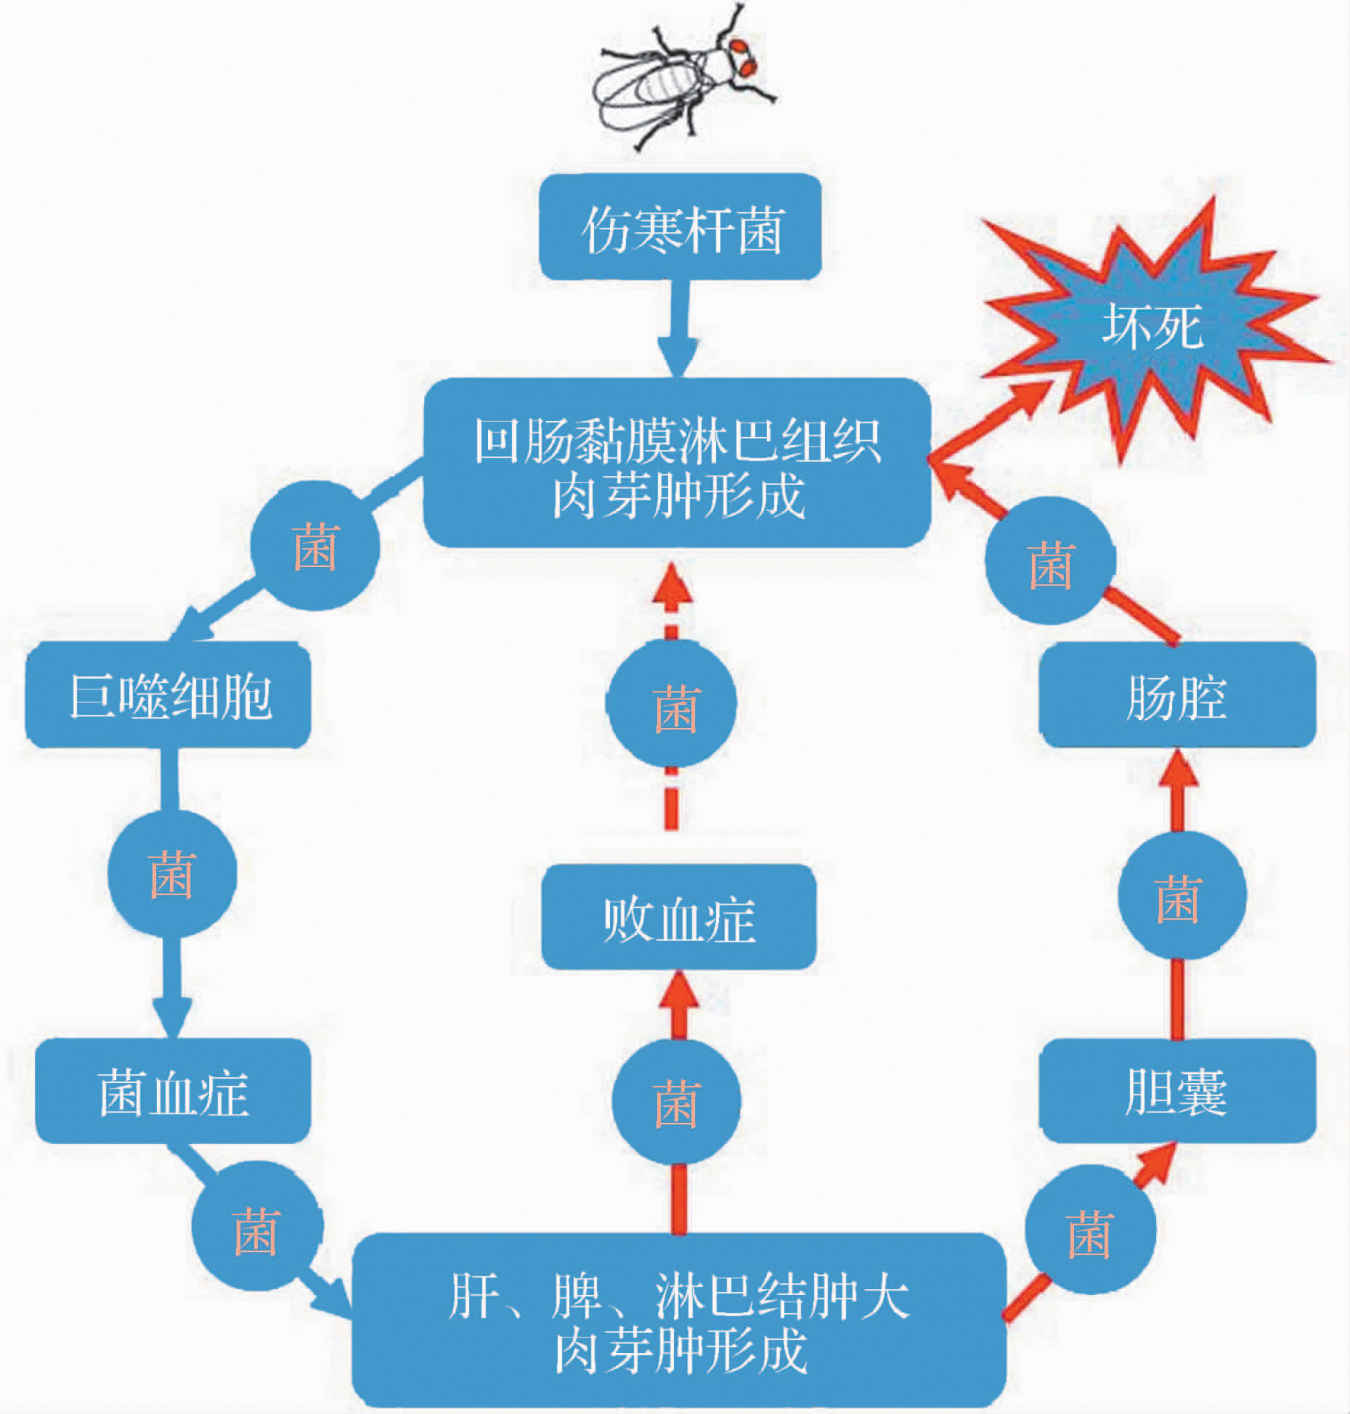
\includegraphics{./images/Image00235.jpg}
    \captionsetup{justification=centering}
    \caption{伤寒病发病机制示意图}
    \label{fig14-10}
\end{figure}

\subsection{病理变化及临床病理联系}

伤寒病变特征为全身单核巨噬细胞增生为主的急性增生性炎。增生的巨噬细胞体积大,具有活跃的吞噬能力,胞浆中常吞噬有伤寒杆菌、红细胞、淋巴细胞和坏死细胞的碎屑等,这种细胞称为伤寒细胞(typhoid
cell)。伤寒细胞常聚集成团,形成境界清楚的结节样病灶,称为伤寒小结或伤寒肉芽肿(typhoid
granuloma)(图\ref{fig14-11}),具有病理诊断价值。

\begin{figure}[!htbp]
    \centering
    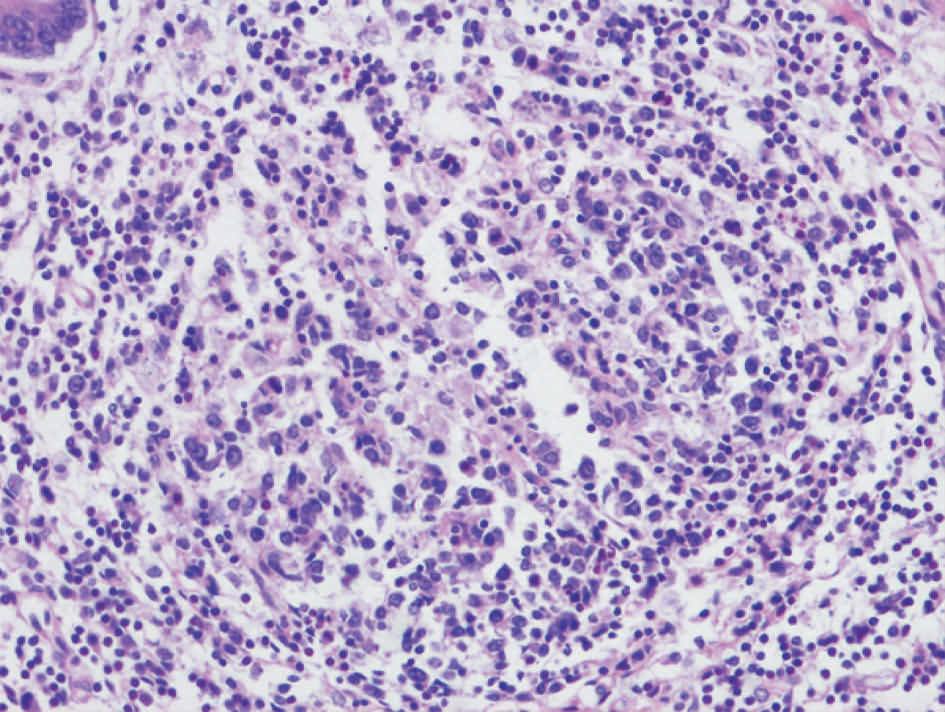
\includegraphics{./images/Image00236.jpg}
    \captionsetup{justification=centering}
    \caption{伤寒肉芽肿:由吞噬了伤寒杆菌、衰老红细胞、淋巴细胞和组织碎屑的伤寒细胞组成(HE染色,中倍)}
    \label{fig14-11}
\end{figure}

\subsubsection{肠道病变}

病变主要发生在回肠下段孤立和集合淋巴小结。按病变自然发展过程分为四期,每期大约持续一周(图\ref{fig14-12})。

\begin{figure}[!htbp]
    \centering
    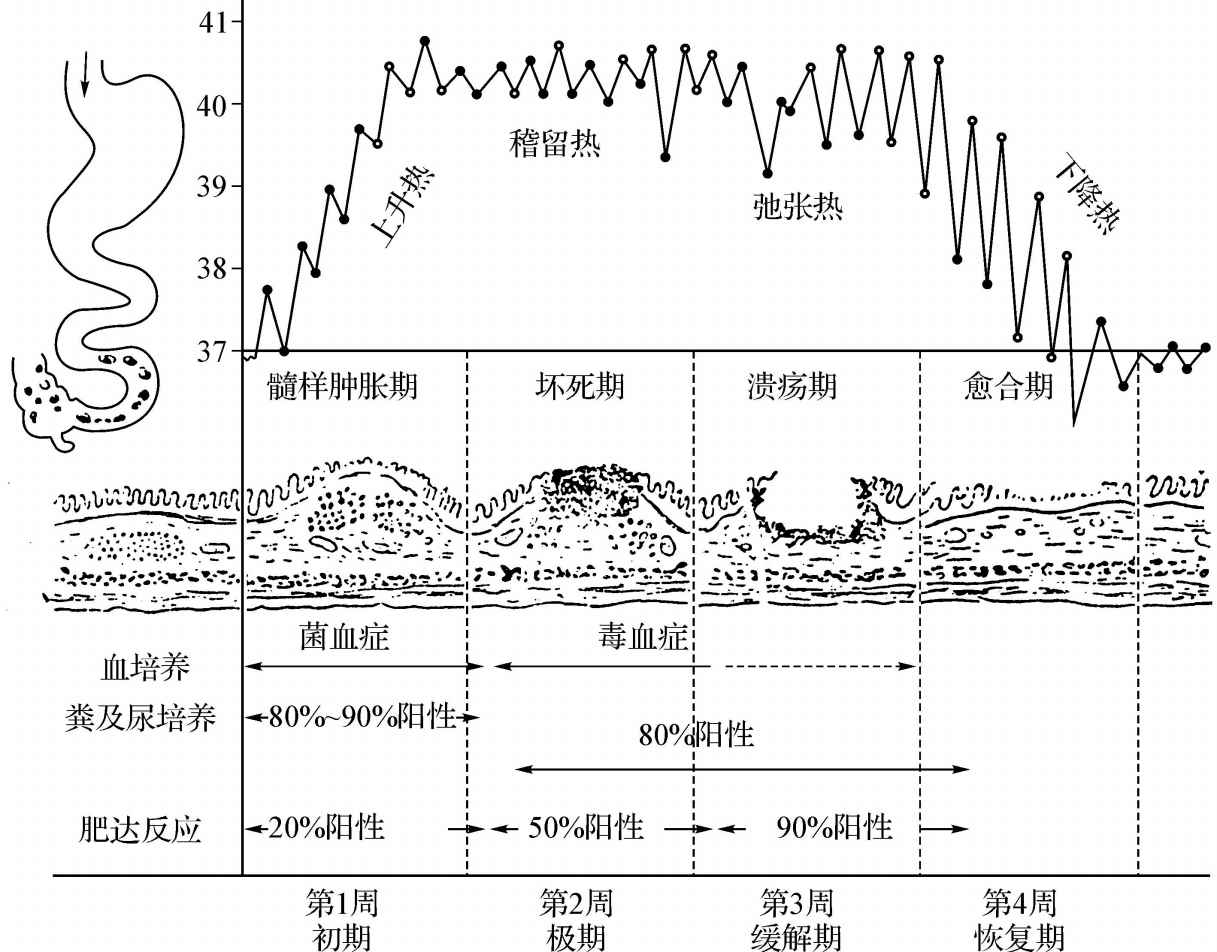
\includegraphics[width=.6\textwidth]{./images/Image00237.jpg}
    \captionsetup{justification=centering}
    \caption{伤寒病肠道病变发展与临床表现的关系}
    \label{fig14-12}
\end{figure}

\paragraph{髓样肿胀期}
起病第一周,肉眼观:肠壁充血、水肿、增厚。孤立与集合淋巴小结增生、肿胀,呈圆形隆起于黏膜表面,灰红色,质软,表面凹凸不平,形似脑回故称“髓样肿胀”,以集合淋巴小结最为典型,愈近回盲部病变愈显著(图\ref{fig14-13})。镜下观:肠壁淋巴组织中有大量增生的伤寒细胞并形成伤寒肉芽肿。此外,肠壁水肿、充血,有淋巴细胞及浆细胞弥漫浸润,但无中性白细胞浸润,这是伤寒杆菌所致炎症的特点。

\begin{figure}[!htbp]
    \centering
    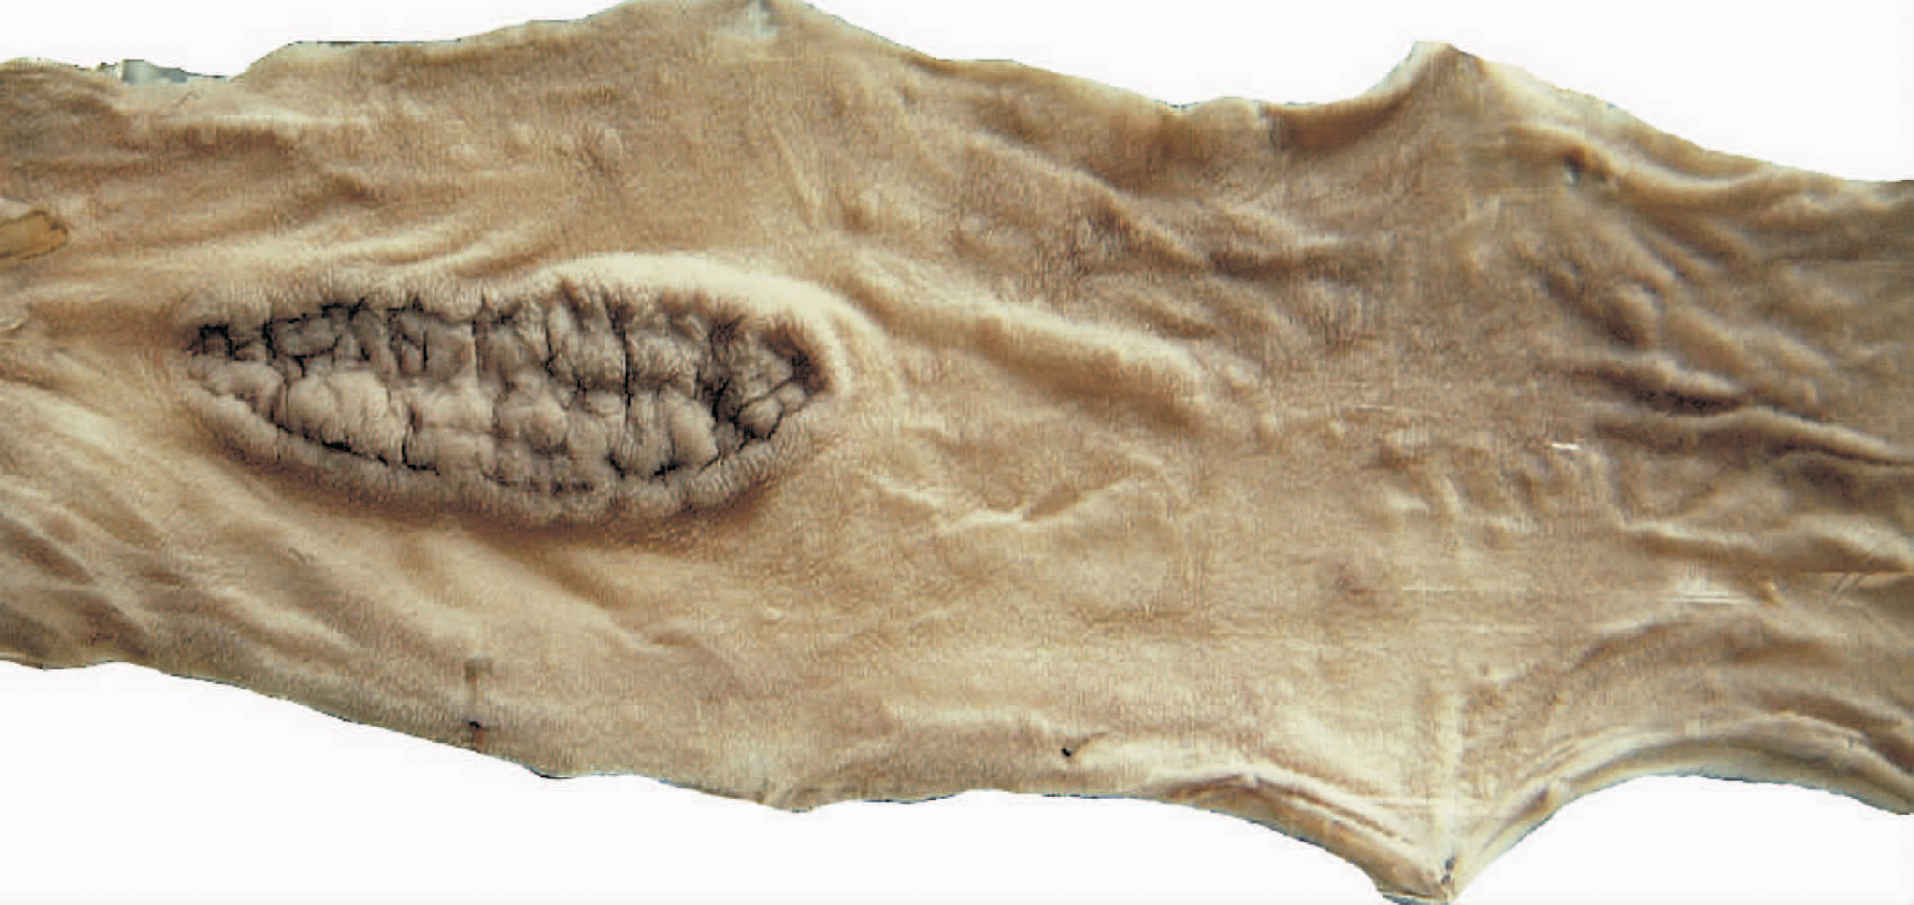
\includegraphics{./images/Image00238.jpg}
    \captionsetup{justification=centering}
    \caption{肠伤寒髓样肿胀期\\ {\small 回肠集合淋巴小节肿胀呈草鞋底样外观}}
    \label{fig14-13}
\end{figure}

此期由于毒血症逐渐加重,病人体温呈阶梯状上升,数日内即达40℃以上,伴有头痛、咽痛、四肢酸痛乏力、全身不适、食欲减退。因巨噬细胞增生,故淋巴结、肝、脾肿大。血及骨髓细菌培养阳性率高。

\paragraph{坏死期}
相当于起病后第二周。由于肠壁淋巴组织发生强烈的过敏反应,加之细菌内毒素作用和伤寒细胞大量增生,压迫毛细血管或血管内有血栓形成,阻塞血流,使局部缺血,导致髓样肿胀的淋巴组织从中心开始发生小灶性坏死,并逐渐扩大融合。坏死表面粗糙,高低不平,灰白色无光泽,有时也可被胆汁染成黄色。

此期患者毒血症状加剧,高热持续不退,稽留在40℃左右。由于病原菌内毒素作用于中枢神经系统,可出现嗜睡、表情淡漠、反应迟钝的无欲貌(伤寒面容),重者更有谵妄、神志不清、昏迷或脑膜刺激症状。肝、脾肿大,粪尿细菌培养可出现阳性,补体结合凝集效价逐渐升高,血象中白细胞减少,嗜酸性粒细胞减少或消失,贫血较常见。部分患者一般在发病10日内,在胸、背和腹部分批出现淡红色、直径在2~4
mm、压之褪色的斑丘疹即玫瑰疹,主要是皮肤的毛细血管被伤寒杆菌栓塞,引起小灶性炎症和毛细血管扩张充血所致,皮疹中可查见或培养出伤寒杆菌。玫瑰疹经3~5天即自行隐退。

\paragraph{溃疡期}
相当于起病后第三周。坏死肠黏膜逐渐崩解脱落形成溃疡。溃疡常为多灶性,边缘隆起,底部高低不平,在集合淋巴小结发生的溃疡较大,呈椭圆形,溃疡长轴与肠的长轴平行。孤立淋巴小结溃疡小,呈圆形。溃疡深浅不一,常达黏膜下层,严重者可达肌层甚至浆膜层可引起穿孔,如累及血管引起肠出血。

此期随着人体免疫力增强,机体逐渐产生抗体,肥达反应滴定度逐渐升高,血培养渐转阴性,但粪、尿培养常常呈阳性。临床体温明显波动呈弛张热型,中毒症状减轻。但此期肠道病变的严重程度与临床症状轻重不完全一致,容易引起并发症,体温骤降或脉率增快为危险并发症(如出血、穿孔)的先兆。

\paragraph{愈合期}
相当于起病第四周。随坏死组织完全脱落,从底部长出肉芽组织,将溃疡逐渐填平,并由溃疡边缘的上皮再生覆盖而愈合。一般不留瘢痕,较大而深的溃疡虽形成瘢痕,一般不会造成肠腔狭窄。

此期患者病情好转,体温呈阶梯状下降,临床症状消失,一般在一个月左右完全恢复。

\subsubsection{其他组织病变}

\paragraph{肠系膜}
淋巴结、脾、肝及骨髓内巨噬细胞增生活跃而致相应组织器官增大,伤寒肉芽肿形成,严重者可有灶状坏死。

\paragraph{心肌}
心肌纤维水样变性,严重的病例可发生心肌坏死及中毒性心肌炎,心肌收缩力减弱。临床上出现重脉或相对缓脉,可能是由于内毒素对心肌的影响和迷走神经兴奋性增高所致。

\paragraph{中枢神经系统}
细菌可引起脑的小血管内膜炎,脑神经细胞变性、坏死以及胶质细胞增生。

\paragraph{其他}
肾脏、皮肤可出现水样变性及玫瑰疹;膈肌、腹直肌和股内收肌常发生凝固性坏死(蜡样变性),可出现肌痛和皮肤知觉过敏。

\subsection{结局和并发症}

\subsubsection{结局}

在无并发症的情况下,一般经过4~5周的自然病程即可痊愈。病后可获得较强的免疫力。自从应用抗生素治疗伤寒以来,典型伤寒病变已较少见,临床表现减轻,病程缩短,并发症减少,但复发率却有所增加。这可能是由于治疗不彻底或免疫力不稳固,尤其是细胞免疫功能不足时,体内没有完全杀死的病原菌,可再度繁殖并侵入血流而引起复发。

\subsubsection{并发症}

伤寒如不出现并发症,一般经过4~5周即可痊愈。严重的毒血症、肠出血和肠穿孔是本病的主要死亡原因。

\paragraph{肠穿孔}
多发生于溃疡期,是伤寒最重要的并发症。肠穿孔可大可小,常为多个,有时为单个,穿孔后可导致弥漫性腹膜炎。

\paragraph{肠出血}
是伤寒常见的并发症。常发生于坏死期或溃疡期,严重者可发生出血性休克。

\paragraph{支气管肺炎}
以小儿患者多见,常是由于机体抵抗力降低,肺炎球菌或其他呼吸道细菌感染所致,极少由伤寒杆菌本身引起。

\section{细菌性痢疾}

细菌性痢疾(bacillary
dysentery)是由痢疾杆菌引起的一种肠道传染病,简称菌痢。基本病理变化为结肠纤维素性炎。临床表现有腹痛、腹泻、里急后重、黏液脓血便和全身毒血症状。本病全年都可发生,以夏秋季为多见,多为散发,也可引起流行。儿童发病率较高。

\subsection{病因及发病机制}

痢疾杆菌为革兰染色阴性杆菌,分为福氏(Flexner)、宋氏(Sonne)、鲍氏(Bogd)和志贺氏(Shiga)痢疾杆菌。所有痢疾杆菌均能产生内毒素,志贺菌还可产生外毒素。我国流行的菌痢主要由福氏菌和宋氏菌引起。

患者和带菌者是传染源。含菌的粪便可直接或间接(通过苍蝇等)污染食物、饮水、用具和手,再经口传染给健康人。多散发,偶可引起暴发流行。

痢疾杆菌进入人体后是否发病,是与细菌的数量多少和毒力大小、肠道防御功能和全身抵抗力的强弱有关。经口入胃的痢疾杆菌可被胃酸杀灭不发病。只有少量细菌进入肠道后,机体全身或局部抵抗力降低时,如过度疲劳、暴饮暴食和胃酸缺乏等,痢疾杆菌才能侵入肠黏膜上皮细胞内生长繁殖,然后通过基底膜进入黏膜固有层,并在该处继续生长繁殖,产生毒素,迅速引起肠黏膜炎症和全身毒血症。

\subsection{病理变化及临床病理联系}

菌痢的主要病理变化在结肠,尤以直肠和乙状结肠为重。病变严重者可波及整个结肠甚至回肠下段。根据病变和临床经过不同可把菌痢分为以下三种类型。

\subsubsection{急性细菌性痢疾}

急性菌痢的典型病变是初期为急性卡他性炎,随后是特征性假膜性炎。

\paragraph{病理变化}
病变初期为急性卡他性炎,表现为结肠黏膜及黏膜下层充血、水肿、中性粒细胞浸润和黏液分泌增多,整个肠壁增厚,并伴有黏膜出血。病变进一步发展形成本病特征性假膜性炎,表现为黏膜表层坏死,有大量纤维蛋白渗出,坏死组织同渗出的纤维蛋白和中性白细胞、红细胞、细菌在黏膜表面形成灰白色糠皮样假膜(图\ref{fig14-14})。发病一周左右,假膜开始脱落,形成大小不等、形状不规则的地图状浅表溃疡。炎症消退后,溃疡由黏膜上皮再生修复愈合,不留明显瘢痕,不引起肠腔狭窄。

\begin{figure}[!htbp]
    \centering
    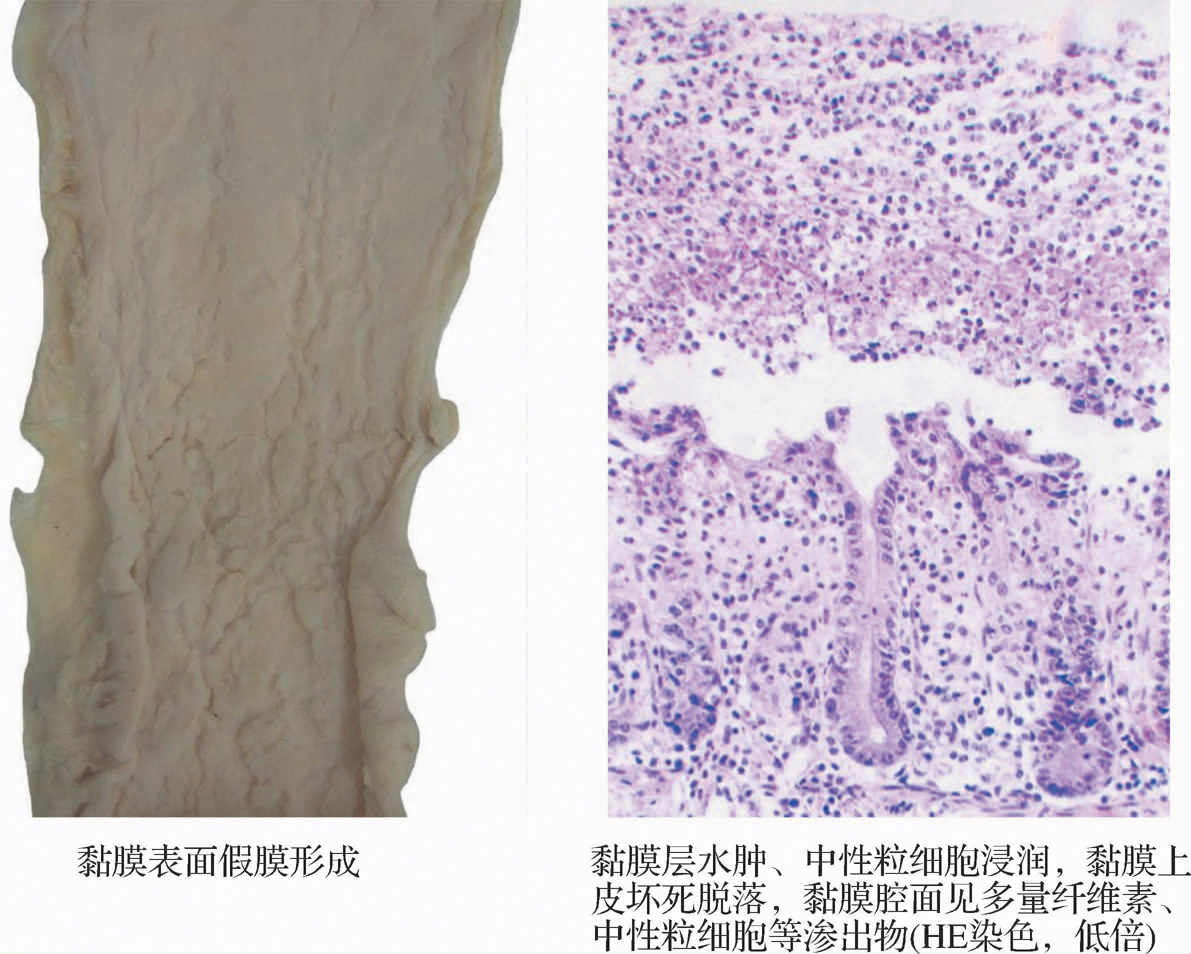
\includegraphics{./images/Image00239.jpg}
    \captionsetup{justification=centering}
    \caption{细菌性痢疾}
    \label{fig14-14}
\end{figure}

\paragraph{临床病理联系}
由于毒血症,可引起发热、全身不适、食欲减退、白细胞增高等全身症状。由于局部炎症刺激,肠蠕动亢进、肠肌痉挛、腺体分泌亢进以及对水分吸收障碍,引起阵发性腹痛、腹泻等症状。初起为水样便和黏液便,系肠黏膜的卡他性炎,由于分泌大量黏液和浆液所致;随着肠道炎症变化,以后转为黏液脓血便,系假膜脱落形成溃疡,导致黏膜出血和脓性渗出的结果;因直肠和乙状结肠病变较重,故腹痛主要在左下腹;炎症刺激直肠内的神经末梢及肛门括约肌,导致里急后重和排便次数频繁。急性菌痢的病程一般1~2周,经适当治疗大多数痊愈。并发出血、肠穿孔少见,少数可转为慢性。

\subsubsection{慢性细菌性痢疾}

急性菌痢未及时彻底治疗,病程超过两个月以上者称为慢性菌痢。以福氏菌感染转变为慢性者多见。有的病程可长达数月或数年。病变特点是肠道病变新旧并存,原有病变尚未完全愈合,而新的病变又可发生。肠道溃疡一般不规则、较深、可达肌层,底部凹凸不平,有肉芽组织和瘢痕形成,溃疡边缘黏膜常过度增生形成息肉。由于溃疡和修复反复交替进行,使肠壁不规则增厚、变硬。严重者可造成肠腔狭窄。

临床上由于肠道慢性炎症引起肠功能紊乱,可出现腹痛、腹胀、腹泻或腹泻与便秘交替出现,粪便中常带有黏液或少量脓血便。在急性发作时可出现急性菌痢症状。有少数患者可无明显症状或体征,但大便培养持续阳性,成为慢性带菌者,是菌痢传播的重要传染源。

\subsubsection{中毒性细菌性痢疾}

多见于2~7岁儿童,成人很少见。其特征是起病急骤,全身中毒症状重而肠道病变和症状相对轻微。患者于发病后数小时即可出现中毒性休克,导致脑组织微循环障碍、脑缺氧、脑淤血和脑水肿改变,引起颅内压升高,甚至脑疝形成,致使呼吸、循环衰竭而死亡;肠道病变不明显,很少形成假膜和溃疡,故临床上常无明显腹痛、腹泻和脓血便。

中毒性菌痢常由毒力较低的福氏或宋氏痢疾杆菌引起,而毒力强的志贺氏菌反而少见。其发病机制尚未明确,可能与患者特异体质或小儿的神经系统发育不完全、功能不稳定而对细菌毒素呈强烈的过敏反应有关。可见其发病主要取决于机体的反应性。

\subsection{结局及并发症}

急性菌痢经治疗后大多能痊愈。部分慢性菌痢可反复发作或成为慢性带菌者。极少数患者出现肠出血、肠穿孔、肠狭窄及支气管性肺炎。中毒性菌痢死亡率较高,必须及时抢救。

\section{性传播疾病}

性传播疾病(sexually transmitted
disease,STD)是以性接触为主要传播途径的一类传染病。传统的性疾病包括梅毒、淋病、软下疳、性病性淋巴肉芽肿和腹股沟肉芽肿五种。近十年STD谱增宽,其病种已多达20余种。本节主要叙述尖锐湿疣、淋病、梅毒和艾滋病。

\begin{framed}
    {案例14-2}

    {【病例摘要】}

    某男,65岁。搬重物时,突然死亡。尸体解剖发现:升主动脉根部膨隆,局部有一0.5
    cm破裂口,胸腔大量积血;主动脉瓣关闭不全;肝、脾切面见散在结节状病灶,直径0.5~2
    cm不等,质韧。镜下见主动脉壁弹力纤维断裂,肝、脾有树胶样肿形成,病变组织易见动脉内膜炎及血管周围炎改变,伴淋巴细胞、巨噬细胞和浆细胞浸润。根据所给病史和尸检结果,回答下述问题。

    {【问题】}

    (1)该患者最有可能患哪种疾病?病因是什么?

    (2)传播途径是什么?疾病的发展过程如何?
\end{framed}

\subsection{尖锐湿疣}

尖锐湿疣(condyloma
acuminatum)是由人乳头状瘤病毒(HPV)感染引起的性传播疾病。发病年龄高峰在20~40岁。免疫组化法检测乳头状瘤病毒核壳抗原及运用原位杂交技术检测HPV的DNA,阳性者有助诊断。

\subsubsection{病因及发病机制}

本病主要由HPV
6型、11型引起。HPV属DNA病毒,只侵袭人体皮肤和黏膜。主要通过性传播,也可通过间接途径,如浴巾、浴盆传染,潜伏期通常为3个月。

\subsubsection{病理变化及临床病理联系}

病变部位,男性常见于阴茎冠状沟、龟头、尿道口或肛门附近。女性常发生在阴蒂、阴唇、会阴、尿道口、宫颈和肛门周围。

肉眼观:早期形成散在小而尖的乳头,逐渐增大增多,呈淡红色或灰白色,质较软,湿润;晚期表面凹凸不平,互相融合形成鸡冠状突起,呈暗红色或污灰色,顶端可因感染而溃烂,根部有蒂,触之易出血。

镜下观:表皮呈疣状或乳头状增生,上皮脚延长、增宽甚至呈假上皮瘤样改变。表皮角化层细胞增生并角化不全,棘层细胞层次增厚。最具有诊断价值的是颗粒层和棘层上部出现大量上皮细胞的核增大,染色质深染,核边缘不整齐,呈轻度异型性,核周有空晕,整个细胞呈空泡状的凹空细胞(挖空细胞)(图\ref{fig14-15})。真皮层毛细血管扩张,有不等量的慢性炎细胞浸润。临床表现局部瘙痒、烧灼痛等。

\begin{figure}[!htbp]
    \centering
    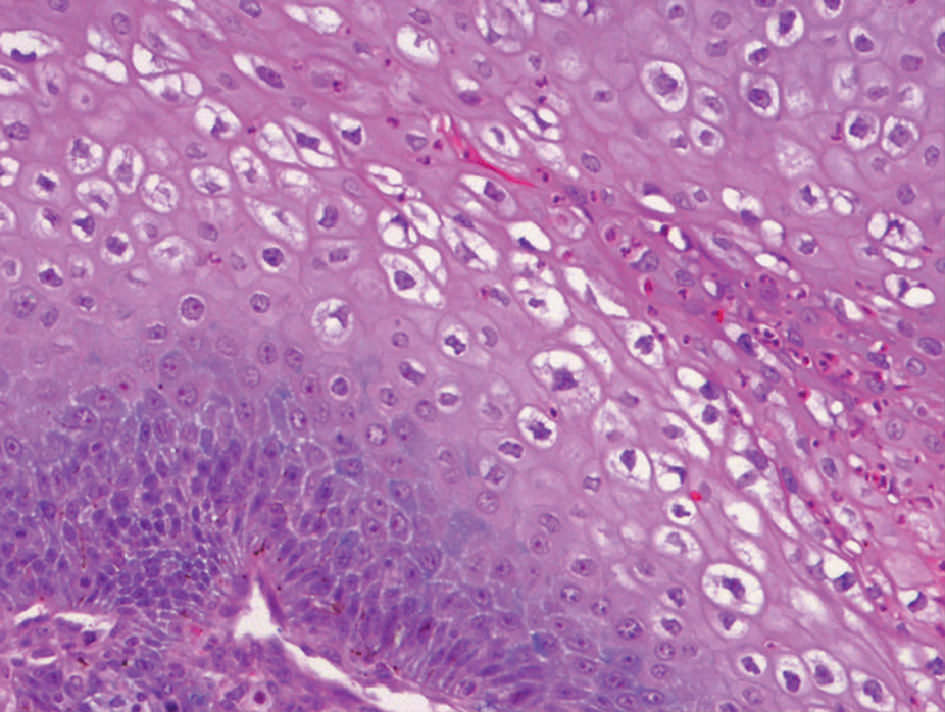
\includegraphics{./images/Image00240.jpg}
    \captionsetup{justification=centering}
    \caption{尖锐湿疣组织形态(HE染色,高倍)\\ {\small 图中可见较多凹空细胞}}
    \label{fig14-15}
\end{figure}

\subsection{淋病}

淋病(gonorrhea)是由淋球菌引起的一种最常见的性传播疾病。以侵犯泌尿生殖系统黏膜为主的一种急性化脓性炎,多发生于15~30岁年龄段,以20~24岁多见。男性的病变开始于前尿道,可逆行蔓延至后尿道,波及前列腺、精囊和附睾。女性的病变常累及外阴和阴道的腺体、子宫颈黏膜、输卵管及尿道。人是淋球菌唯一天然宿主。

\subsubsection{病因及发病机制}

淋病的病原体是淋球菌,淋球菌为革兰阴性双球菌,菌体和荚膜蛋白具有特异性抗原,菌毛还有侵袭黏膜细胞和抗吞噬作用。本病主要通过直接接触传染,成人的淋病几乎全部通过性交而传染。间接传染很少见,主要是通过患者用过的衣物等传染。患淋病产妇,其胎儿经产道娩出时,可被感染而患淋病性眼结膜炎。淋球菌主要侵犯泌尿生殖系,对单层柱状上皮细胞和移行上皮细胞有特别的亲和力。其侵入过程包括与生殖道上皮的黏附和侵入两个步骤。被柱状上皮细胞吞噬的淋球菌,进入细胞后大量繁殖,导致细胞损伤崩解,然后转致黏膜下层引起炎症反应。这个过程与淋球菌菌体成分以及所分泌的蛋白酶、内毒素和抑制噬中性白细胞、补体等作用有关。

\subsubsection{病理变化和临床病理联系}

成人外阴和阴道鳞状上皮能抗拒淋球菌侵入,但淋球菌易侵犯泌尿生殖系黏膜柱状上皮和移行上皮,一般在感染后第2~7天,局部出现急性化脓性炎;脓性渗出物中有大量中性白细胞,胞质内找到革兰阴性双球菌是诊断的主要依据。

\paragraph{局部病变}
(1)男性淋病:初起病为尿道感染,病变主要位于前尿道,表现为尿道口有脓性渗出物流出,充血水肿,有尿道刺激症状和排尿困难,继而病变上行波及后尿道、膀胱、前列腺、精囊、附睾等。如治疗不彻底或反复感染,机体抵抗力下降,淋球菌产生抗药性等因素可转化为慢性化脓性炎,使组织损伤加重,久之尿道炎性瘢痕形成,可引起尿道狭窄、尿路梗阻、排尿困难等。

(2)女性淋病:主要表现为淋球菌性尿道炎和宫颈炎。尿道炎的症状轻、病程短,但易累及尿道旁腺、前庭大腺而发生急性化脓性炎和脓肿形成,病变部位充血、水肿,有大量脓性渗出物。尿道口有溢脓,甚至脓痂堵塞尿道口。炎症可向上蔓延到宫颈、子宫内膜、输卵管和卵巢,患者表现为阴道分泌物增多及下腹坠胀痛、外阴红肿等。

(3)婴儿淋病:最常见为新生儿淋球菌性眼结膜炎,一般于出生后4天以内出现症状。起病急,可双眼同时受累,多为新生儿经母体产道感染引起的。严重时炎症可穿通角膜导致失明。

\paragraph{全身播散}
淋病除发生泌尿生殖系统病变外,还可通过生活接触污染,或经血行播散引起身体其他部位病变。有1%~3%的患者发生淋球菌性败血症,可伴发急性心内膜炎和脑膜炎。

\subsection{梅毒}

梅毒(syphilis)是由梅毒螺旋体引起的一种慢性传染病。一般通过性交传染,流行于世界各地,是一种常见的STD。新中国成立后,采取了一系列的防治措施,曾基本消灭了梅毒,但近年来,随着国内外人口流动量剧增,在全国各地本病时有发现,尤其在沿海城市有流行趋势,应提高警惕,予以重视。

梅毒病原体侵入机体后,经淋巴管迅速播散全身引起多器官病变,也可以通过胎盘传染给胎儿引起先天性梅毒。本病特点是病程长,呈慢性经过,可侵犯任何器官,其病理变化和临床表现复杂多样,也可隐匿多年而毫无临床表现。基本病理特点是闭塞性动脉内膜炎和结核样肉芽肿(树胶肿)形成。晚期患者可因心、脑血管等重要脏器病变而死亡。

\subsubsection{病因及发病机制}

梅毒的病原体是苍白螺旋体(亦称梅毒螺旋体),在暗视野显微镜下观察,其外形显示均匀螺旋状,在组织切片上不能用常规染色法显示,需要特殊的镀银染色法或免疫荧光检查。梅毒螺旋体在体外的活力低,对理化因素的抵抗力弱,对青霉素、四环素、汞、砷、铋剂敏感。

梅毒患者为唯一的传染源,主要通过性接触方式传染,少数可因输血、接吻或皮肤直接接触传染。此外,梅毒螺旋体可经患病孕妇的血液经胎盘传染给胎儿引起先天性梅毒。

机体在感染梅毒后6周可产生特异性抗体,具有血清学诊断价值。随着抗体的产生,机体对螺旋体的免疫力增强,使病变部位的螺旋体数减少,以至早期梅毒病变可不治自愈的倾向。然而未经治疗或治疗不彻底者,播散在全身的螺旋体常难以完全消灭,这就是复发梅毒及晚期梅毒发生的原因。少数人感染梅毒螺旋体后,在体内可终身潜伏,表现为血清反应阳性,而无病变和临床症状,或在二、三期梅毒时局部病变消失而血清反应阳性者,均称为隐性梅毒。

\subsubsection{基本病理变化}

\paragraph{闭塞性动脉内膜炎及血管周围炎}
小动脉内皮细胞及成纤维细胞增生,管壁向心性增厚,管腔狭窄或闭塞,血管周围炎是指血管周围有单核细胞、淋巴细胞、浆细胞浸润,血管壁可发生坏死,可见于各期梅毒(图\ref{fig14-16})。

\paragraph{树胶肿(gumma)}
病灶为灰白色、境界清楚、大小不等、质地坚韧、略有弹性如树胶故称树胶肿,又称梅毒瘤,是梅毒的特征性病变。镜下结构类似结核肉芽肿,中央为凝固性坏死,类似干酪样坏死,不同于结核结节是坏死不彻底,弹力纤维可保存,类上皮细胞和Langhans巨细胞较少。其周围的小动脉内膜炎和血管周围炎较明显。树胶肿可被吸收、纤维化和瘢痕形成但很少钙化。树胶肿可累及任何器官,是晚期梅毒的特征性病变,最常见于皮肤、黏膜、肝(图\ref{fig14-17})、骨和睾丸。

% here how to make two the graphics aligned at the top?
\begin{figure}[!htbp]
    \centering
    \begin{minipage}[t]{0.48\textwidth}
    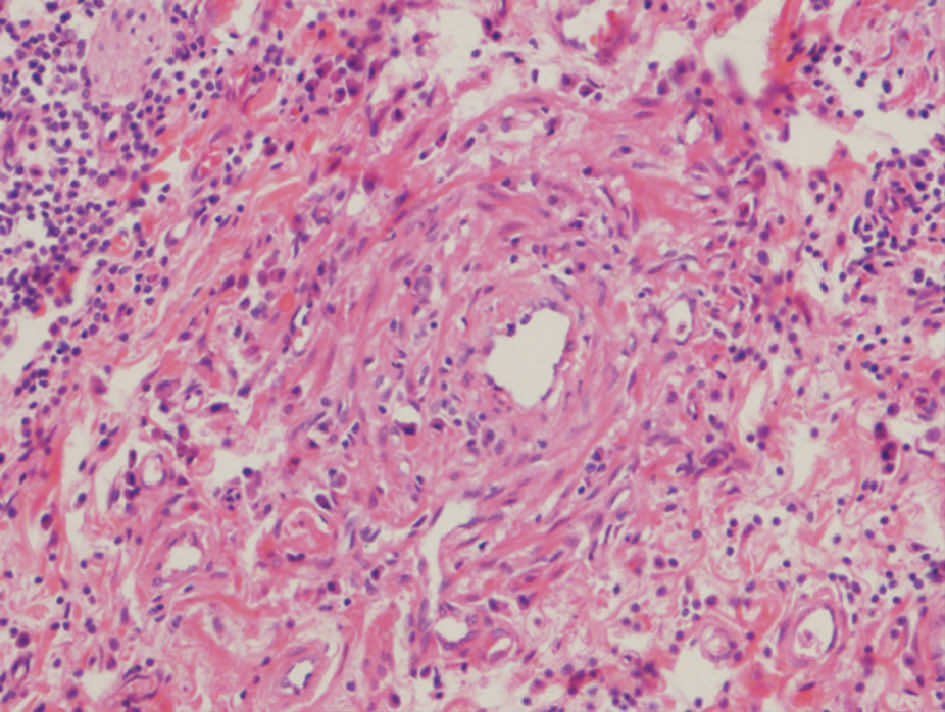
\includegraphics[height=.2\textheight]{./images/Image00241.jpg}
    \captionsetup{justification=centering}
    \caption{梅毒性小动脉炎及血管周围炎(HE染色,中倍)}
    \label{fig14-16}
    \end{minipage}
    %\hspace{0.04\textwidth}%
    \begin{minipage}[t]{0.48\textwidth}
        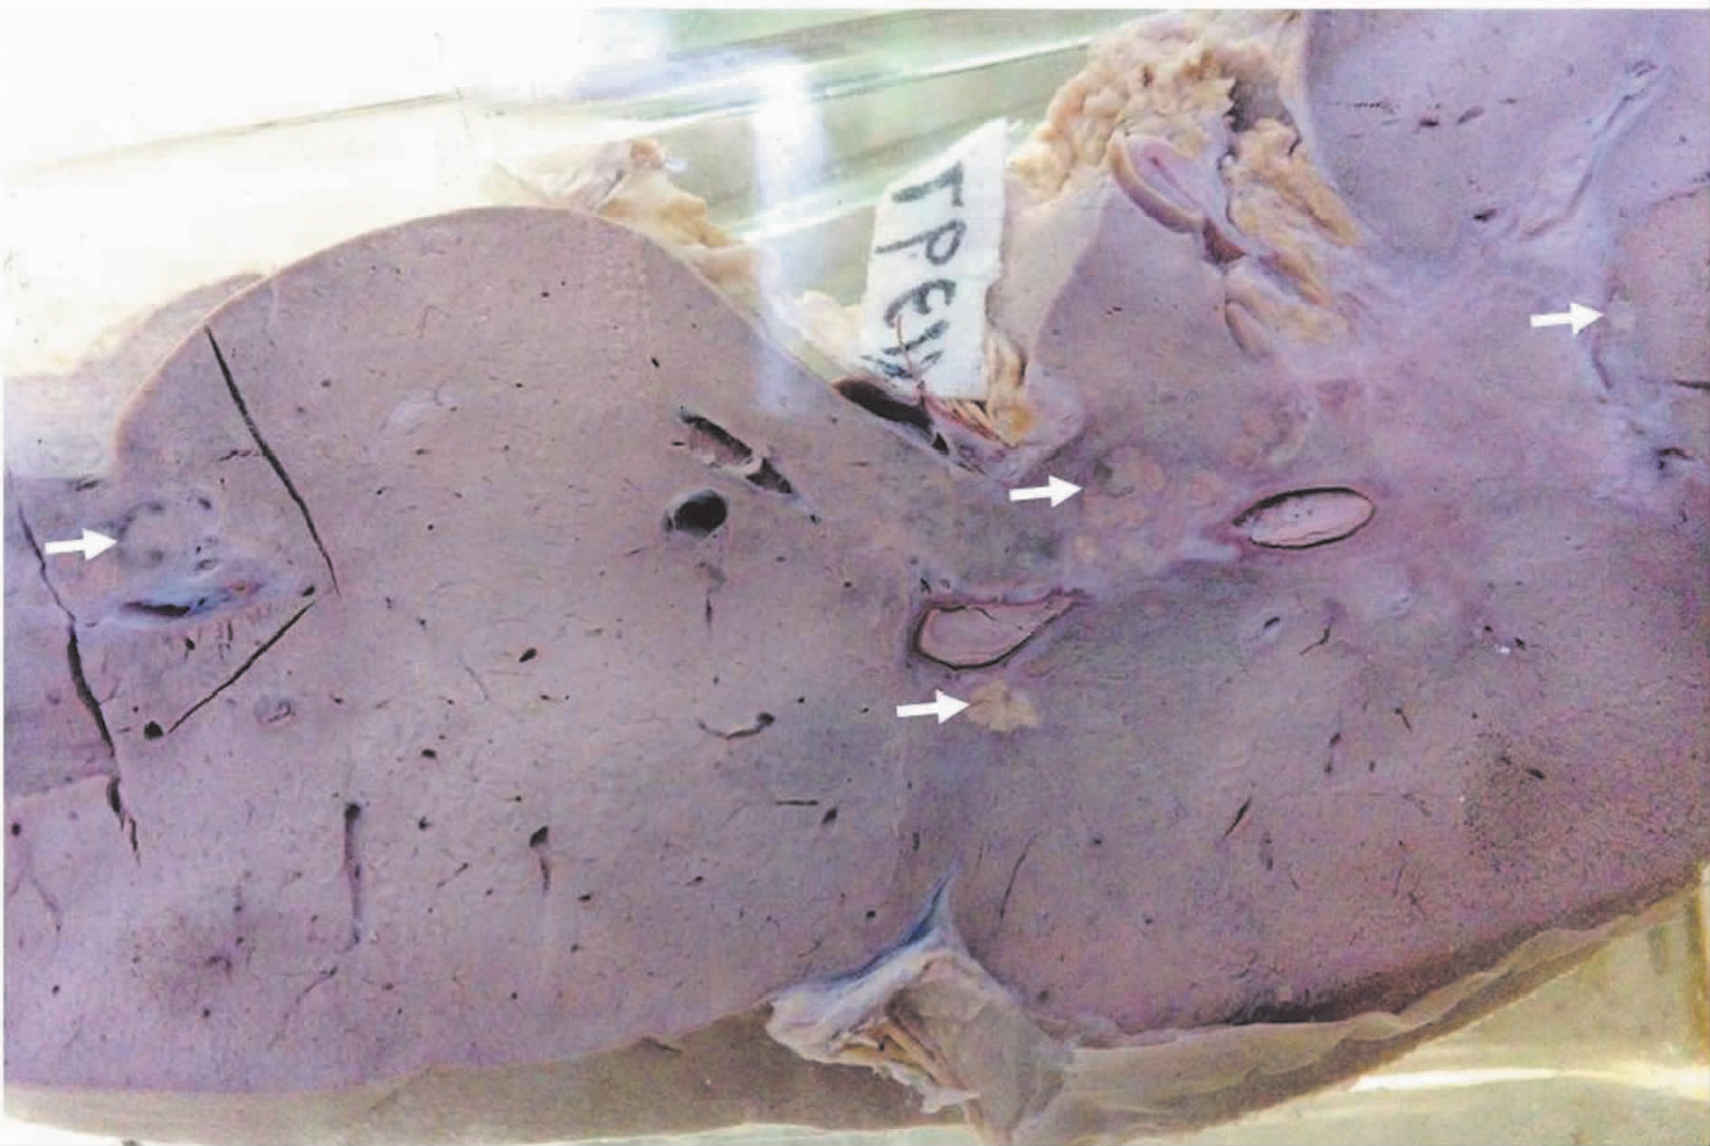
\includegraphics[height=.2\textheight]{./images/Image00242.jpg}
        \captionsetup{justification=centering}
        \caption{肝脏梅毒(白箭头所示为树胶样肿)}
        \label{fig14-17}
    \end{minipage}
\end{figure}

\subsubsection{临床病理类型}

\paragraph{后天性梅毒}
按病变发展过程一般分为三期。其中第一、二期梅毒称早期梅毒,有传染性。第三期梅毒称为晚期梅毒,因常累及内脏,故又称内脏梅毒。

(1)第一期梅毒:梅毒螺旋体侵入人体后三周左右,在侵入部位发生炎症反应,形成下疳。下疳常为单个,直径为1~2cm,表面可有糜烂或溃疡的无痛性硬块,即硬下疳(chancre)。病变多见于阴茎头、子宫颈和阴唇,亦可发生在口唇、舌、肛周等处。镜下为病变处血管周围有大量淋巴细胞和浆细胞浸润,小血管内膜单核细胞浸润,成纤维细胞反应性增生,内皮细胞肿胀,形成闭塞性小动脉内膜炎,病灶内用特殊染色(镀银染色或免疫荧光染色)可查见螺旋体。30%~50%的患者,其下疳太小不易被察觉,或从未发现明显溃疡。下疳出现1~2周后,局部淋巴结肿大,呈非化脓性增生反应。经1个月左右,由于患者产生免疫反应,硬下疳和肿大淋巴结均可不治自愈。临床上处于静止状态,但体内螺旋体仍继续繁殖,如及时治疗可阻止病变向第二期梅毒发展。

(2)第二期梅毒:第一期梅毒如不治愈,在下疳发生7~8周,体内螺旋体大量繁殖进入血循环,引起全身广泛性皮肤黏膜病变,形成各种类型的梅毒疹(syphilid),表现为躯干、四肢弥漫性分布的红色斑疹和丘疹,全身淋巴结肿大。在口唇、会阴或肛周等部位出现暗红色突起的扁平湿疣。梅毒疹镜检所见为闭塞性血管内膜炎和血管周围炎,扁平湿疣则有角化不全和表皮增生。病灶内可检见螺旋体。梅毒疹可自行消退,再次进入无症状的静止状态,但梅毒血清反应阳性。如不治疗,多年后有些患者将发展为第三期。

(3)第三期梅毒:即晚期梅毒,常发生于感染后4~5年,多由于早期梅毒未予治疗或治疗不彻底所致,是梅毒的破坏性病变阶段。病变特点是结节性梅毒疹和树胶肿。病变可累及任何组织和脏器,最常发生于心血管,其次是中枢神经系统。

1)心血管梅毒:病变主要发生于主动脉,引起梅毒性主动脉炎。初起为主动脉外膜滋养血管发生闭塞性内膜炎,导致主动脉中层弹性纤维和平滑肌缺血而发生退行性变和瘢痕化。主动脉瘢痕收缩和内膜纤维组织增生,使内膜表面呈弥漫分布微细深陷的树皮状皱纹(图\ref{fig14-18});如果弹性纤维破坏,在血流冲击下可形成梅毒性主动脉瘤,可因主动脉瘤破裂而猝死;如病变累及主动脉环部,环部弹力纤维破坏,可引起瓣膜环部扩大,加之瓣膜纤维组织增生、收缩、瓣叶间分离,可导致主动脉瓣关闭不全,引起左心室肥大扩张,导致心力衰竭。若主动脉根部瘢痕形成,使冠状动脉内膜增厚、管腔狭窄,由于心肌缺血可发生心绞痛;少数病人可发生梅毒性心肌炎和心包炎,但心肌树胶肿较少见。心血管梅毒是梅毒患者的主要死因。

\begin{figure}[!htbp]
    \centering
    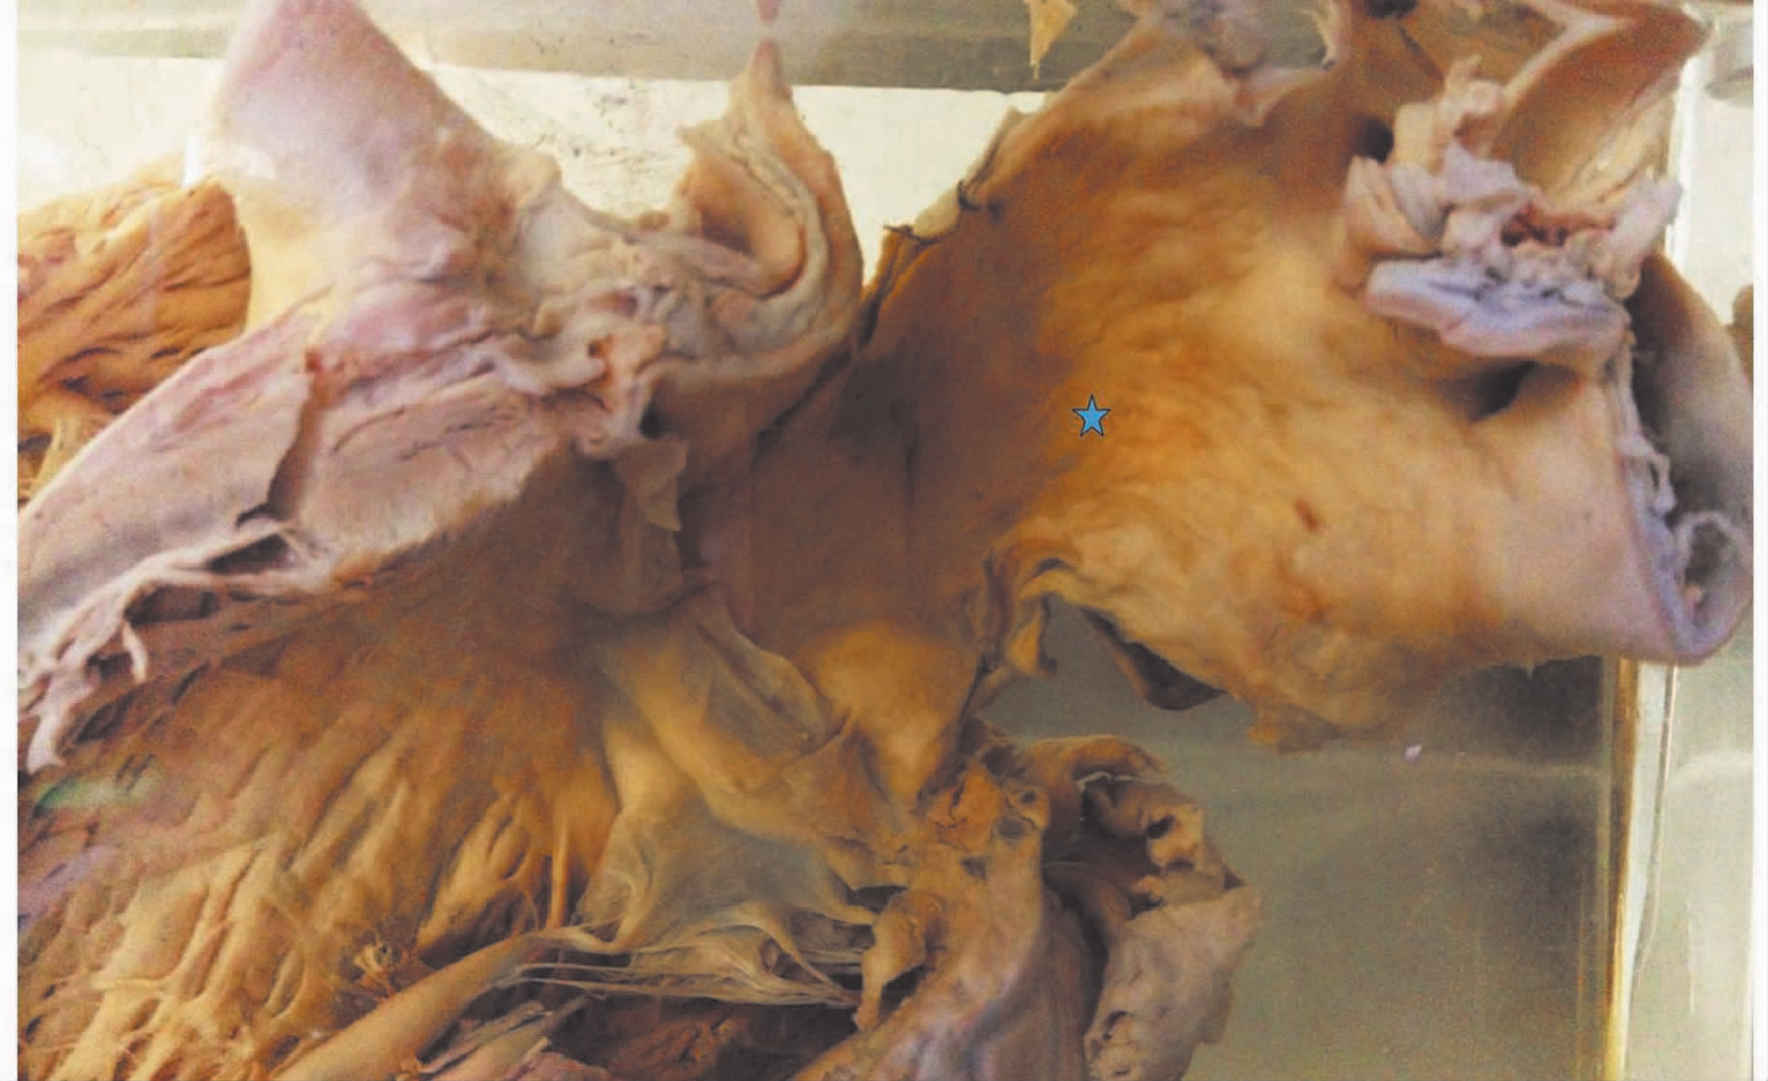
\includegraphics{./images/Image00243.jpg}
    \captionsetup{justification=centering}
    \caption{梅毒性主动脉炎\\ {\small 蓝星所示:主动脉内膜不光滑,呈树皮样改变;同时可见脂斑、脂纹。}}
    \label{fig14-18}
\end{figure}

2)中枢神经梅毒:梅毒螺旋体可侵犯中枢神经及脑脊髓膜,可引起脑膜血管梅毒(脊髓痨和麻痹性痴呆),主要发生于脑底。闭塞性动脉内膜炎导致脑皮质多发性梗死、脑出血;麻痹性痴呆是大脑灰质缺血梗死,尤以额叶的神经元变性、消失伴胶质细胞增生,含铁血黄素沉着所致。临床上常表现为精神失常、性格变化、情绪反常、各种妄想和神经症状,如震颤、癫痫和瘫痪等。脊髓痨是由于脊髓后束和后神经根轴突髓鞘的变性等病变所致。临床表现为共济失调、温痛觉丧失等体征。

3)其他器官梅毒:常见病变为树胶肿。如肝梅毒,树胶肿纤维化引起瘢痕收缩可形成分叶肝。骨梅毒常表现鼻骨、颅骨的坏死崩溃、穿孔,可使鼻梁塌陷,形成所谓马鞍鼻。胫、股骨等亦常易被累及。睾丸梅毒可致不育而且易误诊为肿瘤等。

\paragraph{先天性梅毒}
先天性梅毒是指孕妇血中梅毒螺旋体通过血源途径感染胎儿引起的梅毒。根据被感染胎儿发病早晚不同,先天性梅毒有早发性和晚发性之分。

(1)早发性先天梅毒:系指胎儿或婴幼儿期发病的先天性梅毒(2岁以内发病)。螺旋体在胎儿内脏及组织中大量繁殖,故胎儿和新生儿的皮肤黏膜广泛的梅毒疹形成,重者呈大片剥脱性皮炎。内脏病变表现为淋巴细胞、浆细胞浸润,动脉内膜炎、间质纤维组织增生。骨及软骨等组织也常受累。鼻骨破坏可成马鞍鼻;硬腭破坏可致穿孔;胫骨骨膜炎伴骨膜增生形成新骨,使胫骨向前呈弧形弯曲称为马刀胫。

(2)晚发性先天性梅毒:(指2岁以上发病者)患儿发育不良、智力低下、身材矮小、消瘦、皮肤松弛多皱。除有马鞍鼻、马刀胫外,还可引发间质性角膜炎、神经性耳聋。由于牙齿发育障碍,门齿小而尖,切缘呈镰刀状缺陷,称为何秦森齿(Hutchinson齿)。何秦森齿、间质性角膜炎、神经性耳聋合称为何秦森综合征。是晚发性先天性梅毒的重要特征。皮肤与黏膜病变与成人相似,但不发生硬下疳。

\subsection{获得性免疫缺陷综合征}

获得性免疫缺陷综合征(acquired immunodeficiency syndrome
AIDS)简称艾滋病,是由人类免疫缺陷病毒感染引起的严重免疫缺陷为主要特征的致死性传染病。主要表现为细胞免疫功能低下,使患者失去了对疾病自然抵抗力,从而出现一系列严重的机会感染和恶性肿瘤等。临床常表现发热、消瘦和淋巴结肿大。自1981年首次报告以来,迅速传播,遍及世界各地,死亡率几乎为100%。

\subsubsection{病因及发病机制}

本病病原体是人类免疫缺陷病毒(human immunodeficiency
virus,HIV)。已经在艾滋病病人中分离出HIV-1和HIV-2两种类型病毒。两种病毒引起的病变相似。它存在于患者及无症状HIV感染者的血液中,各种体液如精液、尿液、泪液、唾液、乳头及阴道分泌物、淋巴组织、骨髓、脑脊液中。传播途径多样化,性接触是最常见途径,尤其在男性同性恋中感染率高,其次可通过输入受HIV污染的血液或血液制品、静脉吸毒等途径传染。母体的病毒可经胎盘或哺乳感染胎儿、新生儿。HIV经皮肤或黏膜侵入机体后,随即进入血循环或淋巴系统,能选择性地与CD4{+}
Th细胞表面的受体结合,进入CD4{+}
Th细胞内。病毒在细胞内通常处于不复制的潜伏状态,当受到某种因素激活后开始大量复制,使CD4{+}
Th细胞大量死亡与溶解,导致细胞免疫功能的严重缺陷。同时由于CD4{+}
Th细胞数量减少,失去了对B细胞的辅助作用,当机体免疫功能出现全面缺陷时,机体丧失了对传染病和肿瘤的防御能力,引起严重的机会感染和恶性肿瘤,成为AIDS患者的直接死因。

\begin{center}
    \textbf{知识链接}
\end{center}
\chapterabstract{近年来,艾滋病正从高危人群向普通人群及普通家庭扩散。我国艾滋病流行的主要危险因素为:吸毒、危险性行为(异性性行为和同性性行为)、流动人口、采供血等。少数民族、共用针具、注射吸毒及教育程度≤9年为我国吸毒人群的艾滋病危险因素;甲基苯丙胺、苯丙胺、氯胺酮和摇头丸等人工合成的兴奋剂、致幻剂类毒品为新型毒品,吸毒者容易发生高危性行为,极易造成艾滋病的性传播。中老年嫖客、低档暗娼HIV感染率高;男男性行为人群在我国已成为HIV传播的高危人群。}

\subsubsection{病理变化}

AIDS的病变主要有病毒直接引起淋巴、造血组织和神经系统的原发病变,和由于免疫功能障碍引起的重要器官、组织的机会性感染及恶性肿瘤三方面。

\paragraph{免疫系统原发病变}
(1)淋巴结病变:淋巴组织病变最常见,以淋巴结受损最严重,早期表现淋巴结明显肿大。镜下:起初淋巴结为增生性病变,表现为淋巴滤泡及副皮质区和淋巴窦组织反应性增生,滤泡增大、生发中心活跃,有较多核分裂和巨噬细胞吞噬红细胞现象,淋巴结小静脉也增生。晚期随着病变继续发展,淋巴滤泡开始退化而缩小,生发中心出现萎缩、消失、玻璃样变性,淋巴窦变宽,浆细胞增多,最后T细胞和B细胞区的淋巴细胞普遍减少,甚至完全消失,淋巴结仅剩空架结构,呈现一片荒凉。有些区域结缔组织增生,甚至玻璃样变。淋巴结体积缩小。

(2)脾脏病变:脾脏充血,中度肿大。镜下:主要变化为脾小结明显减少、体积变小,生发中心不明显,中央动脉周围淋巴细胞减少,有较多浆细胞浸润和髓外造血。

(3)骨髓病变:骨髓造血组织中红细胞减少,粒细胞系反应性增生,B淋巴细胞及浆细胞数目增多,并出现异型淋巴细胞,低成熟粒细胞数目下降,提示骨髓造血功能减弱。

(4)胸腺:出现过早萎缩或退化现象,胸腺细胞减少,胸腺小体消失或钙化。

\paragraph{混合性机会感染}
混合性机会感染指在人体免疫功能遭到严重破坏的特定条件下才会引起的感染。常常有两种以上病原体同时感染。其中以呼吸道、消化、中枢神经系统病变最常见。

(1)呼吸道感染:肺是最常侵犯的脏器,约半数的AIDS病患者有卡氏肺囊虫感染,表现为急性重症间质性肺炎,其特征是肺泡腔内出现大量免疫球蛋白和卡氏肺囊虫组成的伊红染色泡沫样渗出物。巨细胞病毒性肺炎亦常见,感染病毒的上皮细胞或血管内皮细胞等体积肿大,核内出现噬伊红染色均质的包涵体,其周围有一圈透亮空晕,胞浆内亦可见成簇的颗粒状包涵体。

(2)神经系统病变:神经系统病变也很重要。80%的尸检材料证实神经系统有多种损害。有人认为HIV是一种亲神经组织的病毒,组织中的单核巨噬细胞和小胶质细胞均是HIV的靶细胞,HIV有可能通过单核巨噬细胞进入血脑屏障,随之侵入中枢神经组织。临床13%~20%的病例以神经系统为首发症状。常见的机会感染有弓形虫、隐球菌或巨细胞病毒引起的脑炎、脑膜炎等,也有HIV直接引起的无菌性脑膜炎、亚急性脑病痴呆、空洞性脊髓病变等。

(3)消化道感染:消化道也是机会感染最常见部位。常见病原体如单纯疱疹病毒、巨细胞病毒、隐球菌、溶组织阿米巴、沙门氏菌等,都可以引起消化道不同的炎症和病变。患者临床上可表现持续性腹泻或复发性腹泻,并可发生溃疡、出血或穿孔。白色念珠菌则可引起口腔甚至食管感染等。

艾滋病患者除可发生混合性机会性感染外,也易发生上呼吸道感染、肺结核、病毒性肝炎、细菌性痢疾及各种化脓菌感染等。

\paragraph{恶性肿瘤}
艾滋病患者由于免疫功能缺陷,导致免疫监视功能丧失,因而也易并发恶性肿瘤,这也是导致艾滋病患者死亡的常见原因之一。有1/3~1/2的AIDS病患者并发Kaposi肉瘤,它是一种来源于血管内皮细胞的恶性肿瘤,其特点是病情进展快,累及范围广,主要发生于皮肤或黏膜,以下肢最常见,并很快累及淋巴结、肺、肝、脾、胰、肾、膀胱和附睾等部位。肿瘤呈单个或多发性紫红色皮肤、黏膜结节或斑块,边界不清,可发生坏死、破溃和出血。镜下:瘤组织由增生的梭形细胞构成毛细血管样腔隙结构,可见核分裂,腔隙内含有红细胞,可发生纤维化和含铁血黄素沉积,晚期可呈现血管肉瘤的图像。

AIDS预后差、死亡率高,患者大多在发病后2年内死亡。对于AIDS的防治,当前没有有效的疫苗和药物,因此,必须应用目前已掌握知识,大力开展预防措施,这对限制AIDS的传播和流行极为重要。

\section*{复习与思考}

{一、名词解释}

结核结节 原发综合征 结核球 冷脓肿 伤寒肉芽肿 伤寒细胞 硬下疳 获得性免疫缺陷综合征

{二、问答题}

1. 简述结核病的基本病理变化及转归。

2. 区别原发性肺结核病和继发性肺结核。

3. 各型继发性肺结核有何特点?

4.
简述伤寒基本病理变化。肠道病变分几期?各期的病变特点是什么?有哪些并发症?

5. 描述急性菌痢的病理变化,解释其临床病理联系。中毒性菌痢有哪些特征?

6. 简述梅毒、淋病、艾滋病的基本病变及其临床病理联系。

{三、临床病理讨论}

病历摘要:王××,女性,7岁。发热伴头痛、恶心、呕吐6天。在当地乡医院拟诊为“流脑”,经治疗未见好转。近日病情加重,进食后即发生喷射状呕吐。今晨开始神志不清、昏迷,于3月6日急诊入院。

入院体检:体温38.5℃,脉搏102次/分,呼吸26次/分,血压14/9
kPa,急性重病容、消瘦、营养不良、颈项强直,呈轻度角弓反张,两肺闻及湿啰音,肝肿大肋下2
cm。

实验室检查:脑脊液压力高,外观混浊,蛋白含量增加,糖及氧化物含量降低,细胞数960/mm{3}
,淋巴细胞70%,涂片抗酸染色查见结核杆菌。

患者入院后,立即给予对症抗结核治疗,但病情日趋恶化,始终神志不清、昏迷,经抢救无效死亡。

尸检所见:

颅腔:脑脊液混浊,脑膜上散在多量灰白色粟粒大小结节。镜检:蛛网膜下腔内有多量浆液、纤维素和巨噬细胞、淋巴细胞渗出,并可见不典型的结核结节。

胸腔:双侧均可见有少量橙黄色液体,肺门淋巴结肿大如蚕豆大小,切面呈干酪样坏死。两肺满布粟粒样大小灰白色的圆形小结节。右肺上叶下部有一直径1
cm左右灰黄色病灶。镜检有组织坏死,周围有朗格汉斯巨细胞、类上皮细胞及淋巴细胞等形成的结核结节。

腹腔:有橙黄色混浊液体约200
ml。腹膜及腹腔器官如肝、脾等表面均可见灰白色粟粒样结节。

讨论题:

1. 写出本例病理诊断。肺部病变与其他脏器病变有何关系?

2. 以病理所见解释临床上的主要症状和体征。




